% MASTER'S THESIS IN MATHEMATICAL INFORMATION TECHNOLOGY
% Tuomo Sipola
%
% Based on Timo Männikkö's template. 
% Uses latex template by Antti-Juhani Kaijanaho and Matthieu Weber.
%

\documentclass[finnish,logo,nonumbib,nocopyright,lof,pdftex]{gradu2}

\usepackage[utf8]{inputenc}

\usepackage{palatino} % Better font
\usepackage[intlimits]{amsmath} % For better math mode, namely integrals
\usepackage{amssymb} % Math symbols

\usepackage[pdftex]{graphicx} % Pictures
%\usepackage{pdfpages} % For inclusion of the article

\usepackage{hyperref}

% Optional 1,5 point line spacing
%\usepackage{setspace}
%\onehalfspace

% Define our own abbreviations list
\newenvironment{abbrlist}[1]{
  \begin{list}{}{\settowidth{\labelwidth}{\textbf{#1}}
  \setlength{\leftmargin}{\labelwidth}
  \addtolength{\leftmargin}{\labelsep}
  \renewcommand{\makelabel}[1]{\textbf{\hfill##1}}}}%
{\end{list}}

% No spacing with this enumeration
\newenvironment{enumerate_no_space}{
  \begin{enumerate}
  \setlength{\itemsep}{1pt}
  \setlength{\parskip}{0pt}
  \setlength{\parsep}{0pt}}
{\end{enumerate}}

% Remoge pagebackref in the final version
% Add "pagebackref=true" to get page numbers where each reference is used
% Link version for internet viewing
%\usepackage[pdftex,colorlinks=true]{hyperref}

% PDF information tags
\pdfinfo{/Title (WWW-palveluihin kohdistuvien hyökkäysten analyysi ja torjunta) /Author (Joel Lehtonen ja Kristian Siljander) /Subject (Mitähän tähän pitäisi kirjoittaa?) /Keywords (tähän avainsana, toinen, jne.)}

%%% Actual content begins here

\title{Web-palveluihin kohdistuvien hyökkäysten analyysi ja torjunta}
\translatedtitle{Analysis of attacks against WWW services, TODO}

\linja{Mobiilijärjestelmät}

\setauthor{Joel}{Lehtonen}
\setauthor{Kristian}{Siljander}
\yhteystiedot{joel.lehtonen@iki.fi}
\yhteystiedot{kristian.r.r.siljander@jyu.fi}
%\setdate{30}{8}{2008}

\abstract{EEG signals can be analyzed with modern mathematical methods
  in order to separate the most meaningful components from the
  rest. Hilbert-Huang transform is a new method to construct a sharp
  and clean time-frequency spectrum of a nonlinear and nonstationary
  signal. It consists of empirical mode decomposition (EMD), which
  decomposes the signal to intrinsic mode functions (IMF), and Hilbert
  transform, which is used to obtain the spectrum. This method was
  used on EEG data recorded during an oddball paradigm test. The
  subjects consisted of children divided into three groups:
  attention-deficit hyperactivity disorder (ADHD), reading-disabled
  (RD) and control group. Hilbert-Huang transform revealed differences
  between the groups that could not have been obtained using more
  conventional analysis methods. }
\tiivistelma{Aivosähkökäyriä, bzzzz!
}

\avainsanat{aivos\"{a}hk\"{o}, her\"{a}tepotentiaali, Hilbert-Huang-muunnos, empiirinen aaltomuotohajotelma, aika-taajuusanalyysi}
\keywords{electroencephalography, EEG, event-related potential, ERP, mismatch negativity, MMN, Hilbert-Huang transform, HHT, empirical mode decomposition, EMD, time-frequency analysis}

\begin{document}

\def\termlistname{Lyhenteet}
\termlist

\begin{abbrlist}{ANOVA}
\item[OMG] Oh my god
\item[LOL] Lulz
\end{abbrlist}

\mainmatter

% -*- mode: LaTeX; coding: utf-8; -*-

\chapter{Johdanto}

Viime vuosina Web-sovellusten ja -palveluiden suosio ja käyttö ovat
olleet kovassa kasvussa, ja monet näistä ovat nykyisin kriittisiä osia
yhteiskuntamme toimivuuden kannalta. Internetin välityksellä
käytettävien palveluiden tietoturvan ja saatavuuden takaaminen on
tämän johdosta noussut monessa yrityksessä tärkeään rooliin.
Tietojärjestelmien siirtyminen julkishallinnon ja
yritysten erillisverkoista julkiseen Internetiin on vaikuttanut omalta
osaltaan myös siihen, mihin tietoturvahyökkäykset nykyisin
kohdistuvat ja kuinka ne pyritään toteuttamaan.

Hyökkäysten muuttuessa yhä hienostuneimmiksi, eivät perinteiset
tietoturvamenetelmät enää riitä suojaamaan loppukäyttäjiä tai palvelun
ylläpitäjiä. Tästä syystä erilaisten tietoturvaratkaisuiden ympärillä
käy kova kuhina, ja aihepiiri on herättänyt suurta kiinnostusta
tutkijoiden keskuudessa. Erilaisia ratkaisuja, joissa on pyritty
selvittämään tietoturvahyökkäyksiä ja näiden mukana tulevia haasteita,
on lukematon määrä. Haaste on löytää ne menetelmät, jotka oikeasti
toimivat riittävällä tarkkuudella ja nopeudella.

Tietoturvahyökkäysten tunnistaminen perustuu siihen, että
analysoimalla yhtä tai useampaa tapahtumaa pyritään löytämään
viitteitä tapahtuvista hyökkäyksistä. Menetelmät jaetaan kahteen eri
tyyppiin: anomalioiden eli poikkeavuuksien tunnistamiseen
(engl. \textit{anomaly detection}) ja väärinkäytösten tunnistamiseen
(engl. \textit{misuse detection}). Näistä anomalioiden tunnistaminen
perustuu malleihin, joita luodaan järjestelmän, käyttäjän tai verkon
normaalista käyttäytymisestä. Tulevaa liikennettä sitten verrataan 
näin luotuihin malleihin, jolloin opituista malleista poikkeava liikenne
voidaan tunnistaa. Väärinkäytösten tunnistamiseen tarkoitetut järjestelmät 
puolestaan sisältävät joukon kuvauksia eli signatuureja tunnetuista hyökkäyksistä. 
Tuleva liikenne tarkistetaan näitä kuvauksia vastaan, jolloin näitä vastaavat
hyökkäykset tunnistetaan. Hyökkäysten tunnistusjärjestelmät
jaetaan joissakin tapauksissa myös sen mukaan, mistä tutkittava
liikenne on kerätty. Tällöin järjestelmät on jaettu verkkoon
pohjautuviksi (engl. \textit{network based}) ja asiakaspohjaisiksi
(engl. \textit{host based}).

Tässä tutkielmassa tietoturvahyökkäykset pyritään tunnistamaan analysoimalla 
Web-palvelimien tuottamaa tapahtumalokia. Lokista yritetään etsiä ja tunnistaa
poikkeavuuksia normaalin liikenteen joukosta käyttäen diffuusiokuvauksia. Näiden
avulla pystytään helpommin esittämään ja kuvaamaan sellaista materiaalia, joka 
koostuu suuresta määrästä parametreja.

Tutkielman rakenne on seuraavanlainen. Luvussa 2 esitellään yleisellä
tasolla Web-palvelinalustoja, ja käydään läpi Web-palveluiden
erilaisia toteutustapoja. Luku 3 käsittelee perinteisiä
tietoturvahyökkäyksiä, ja luvussa 4 perehdytään uudenlaisiin
Web-ratkaisuihin ja tietoturvahyökkäyksiin, joiden kohteeksi
Web-palvelut nykyisin joutuvat.  Luku 5 sisältää kuvauksen
dynaamisista Web-teknologioista, jotka mahdollistavat suurimman osan
nykyisistä tietoturvahyökkäyksistä, ja luku 6 sisältää katsauksen
tutkimuskenttään liittyvään tutkimukseen.

Luvussa 7 kuvaillaan analyysissa käytetyt menetelmät, ja luvussa 8
esitellään tutkimuksen lähtökohta ja analysoitavan materiaalin rakenne.
Samassa luvussa myös käydään läpi esikäsittelijää,joka on on suunniteltu 
ja toteutettu tätä tutkimusta varten. Esimerkkien avulla esitellään myös 
sovelluksen toimintaa.

Luvussa 9 esitellään saatuja tuloksia kuvaajien avulla, ja
analyisoidaan näitä tarkemmin sekä esitetään mahdollisia syitä
saatuihin tuloksiin. Jatkotutkimuksia ajatellen esitetään
myös parannusehdotuksia. Viimeinen luku sitten sisältää
yhteenvedon koko työstä ja ajatuksia sen onnistumisesta.

% -*- mode: LaTeX; coding: utf-8; -*-

\chapter{Web-palvelut}

Web-palveluilla tarkoitetaan järjestelmiä, jotka kommunikoivat
keskenään käyttäen vakiintuneita Web-tekniikoita. Web-palvelimet eivät
ole riippuvaisia mistään tietystä laitteisto- tai
käyttöjärjestelmäarkkitehtuurista. Web-palveluiden käyttämät
teknologiat eivät sinänsä ole erityisen vallankumouksellisia, mutta
tiedonvaihdon helpottuminen standardien protokollien ja Web:n
hajautetun rakenteen ansiosta on tehnyt Web-palveluista
mielenkiintoisia niin kehittäjien kuin käyttäjienkin
näkökulmasta\cite{javaweb}.

IBM määrittelee WWW-palvelut seuraavasti: ``Web-palvelut ovat
itsenäisiä ja modulaarisia sovelluksia, jotka voidaan julkistaa,
määritellä, paikallistaa ja suorittaa verkon ylitse, yleeensä WWW:n
välityksellä.''\cite[s.4]{websecurity}

Tietoturvan kannalta WWW-palvelut ovat haastavia, koska niitä
käytetään Internetin välityksellä eivätkä ne ole rajoittuneita
esimerkiksi tietyn organisaation lähiverkkoon. Myös osia
WWW-palveluista sijaitsee usein fyysisesti eri paikoissa ja ne
kommunikoivat keskenään Internetin välityksellä.

Tässa luvussa käsitellään komponentteja, joista tämänhetkiset
Web-palvelut koostuvat. Erityistä huomiota on kiinnitetty seikkoihin,
jotka vaikuttavat palvelun tietoturvaan.

\section{Palvelinohjelmistot}

Web-palveluiden toteuttajan näkökulmasta lähin komponentti on
palvelinohjelmisto. Se käsittelee HTTP-kyselyt ja lähettää vastauksina
käyttäjän selaimessa näytettäviä ja prosessoitavia osia, kuten
hypertekstiä, kuvia ja komentosarjoja.

Web-palvelinohjelmisto ei useinkaan kommunikoi suoraan palvelun
käyttäjän tietokoneen kanssa vaan välissä on usein välimuistipalvelu,
joka vähentää palvelimelle kohdistuvaa rasistusta säilyttämällä
harvoin muuttuvaa sisältöä välimuistissa ja välittämällä tätä suoraan
käyttäjille. Muuttuva tai välimuistille uusi sisältö pyydetään
palvelinohjelmistolta.

Internet-tietoturvapalveluita tarjoavan Netcraftin\cite{netcraft}
raportista huhtikuulta 2010 käy ilmi, että kaksi suurinta
Web-palvelinalustaa ovat Apache (53.93\% suosituimmista sivuista),
Microsoft (24.97\%). Näiden jälkeen tulevat Google ja nginx kumpikin 6\%
osuudella.

Tuloksia voi vääristää jonkin verran se, että joissakin tapauksissa
edustalla suoritetaan välimuistipalveluna toista palvelinohjelmistoa,
esimerkiksi Apachea tai nginx:ä, joka välittää kyselyt eteenpäin
varsinaiselle Web-palvelinohjelmistolle. Tämä selittää esimerkiksi
sen, miksi Zope puuttuu kokonaan suosituimpien palvelinten
joukosta. Esimerkiksi Jyväskylän yliopiston Web-palvelimena näkyy
tilastoinnissa Apache, vaikka Web-palvelu on toteutettu
Zope-palvelinohjelmiston päällä suoritettavalla Plonella. Samoin on
käynyt Tomcat-palvelimella ajettavalle Korppi-opintotietojärjestelmälle.

\subsection{Apache}

Suosituimpana palvelinalustana Apache on luonnollisesti suosittu kohde
myös tietomurtojen yrityksille. Apachesta itsestään on kuitenkin
löydetty verrattain vähän
tietoturva-aukkoja.~\cite{apachetietoturva}. Suurin osa tietomurroista
keskittyykin murtamaan varsinaista Web-palvelua palvelinalustan sijaan.

Apache pystyy suorittamaan komentosarjoja perinteisen CGI-rajapinnan
lisäksi myös palvelinlaajennosten avulla, jolloin saavutetaan
tiiviimpi integraatio ja enemmän suorituskykyä verrattuna
CGI-rajapintaan~\cite{cginopeus}.

Apachea voidaan suorittaa lukuisissa eri käyttöjärjestelmissä, joista
Linux on ylesiin~\cite{apachemarket}. Suosittuja Apache-alustalla
käytettäviä ohjelmointikieliä ovat PHP ja Python. Tunnettuja tässä
ympäristössä käytettäviä Web-palveluita ovat mm. Wikipediassa
käytettävä MediaWiki ja lukuisilla selainkäyttöisillä
keskustelupalstoilla käytettävä phpBB.

TODO LAMP (Linux + Apache + MySQL + PHP)

\subsection{Zope}

+Plone. TODO

\subsection{Tomcat}

TODO

\subsection{IIS}

TODO.

\section{Hajautetut palvelut}

TODO Pyynnön ohjaaminen usealle palvelimelle (reverse proxy), Hyödyt verrattuna keskitettyyn

\section{Välimuistipalvelut}

TODO 
- "talon sisällä" olevat välimuistit
 - Akamai ym. "ulkoiset" välimuistit (ei luovuta esim. IP-osoitteita)
 - tiedon keräämisen kannalta IDS:lle (minkälaiset logitukset?)


% -*- mode: LaTeX; coding: utf-8; -*-

\chapter{Perinteiset tietoturvahyökkäykset}

Tietoyhteiskunnassa yksikään verkossa oleva laite ei ole suojassa
tietoturvahyökkäyksiltä, ja niiden mukanaan tuomilta
ongelmilta. Hyökkäykset ovat nykyisin myös hyvin monimuotoisia ja ne
voidaan jakaa eri kategorioihin niiden tavoitteiden ja toteutustapojen
mukaan. Uusia hyökkäystapoja kehitetään jatkuvasti lisää ja
tunnetutkin hyökkäystavat saavat uusia ominaisuuksia. Vaikka
suurimpaan osaan hyökkäyksistä on olemassa erilaisia
suojautumistapoja, on näiltä kaikilta suojautuminen ylläpitäjän
kannalta mahdoton tehtävä. Verkon turvallisuuden kannalta on kuitenkin
tärkeää, että hyökkäysten riskit tiedostetaan ja uhkien toteutumisen
todennäköisyyksiä voidaan pienentää mahdollisuuksien ja resurssien
rajoissa.


\section{Tiedon urkinta ja väärentäminen}

Ennen kuin hyökkääjä pystyy murtautumaan verkkoon tai verkossa
sijaitsevaan tietokoneeseen, tulee hänen selvittää järjestelmän
mahdolliset heikkoudet. Haluttuja tietoja ovat esimerkiksi asennetut
käyttöjärjestelmät, ohjelmistojen versiotiedot sekä verkon yleinen
rakenne ja tietoturvataso. Näiden tietojen selvittämiseksi hyökkääjä
aloittaa verkkoa kohtaan joukon hyökkäyksiä, joita kutsutaan
tiedusteluhyökkäyksiksi (engl. \textit{Probe Attacks}). Tällaiset
tiedustelut ovat varsinaisia hyökkäyksiä yleisempiä, sillä niiden
toteuttaminen ei vaadi hyökkääjältä kovin syvällistä
osaamista. Verkosta löytyy paljon valmiita työkaluja, joiden avulla
hyökkääjä pystyy urkkimaan tarvittavat tiedot ja mahdollisesti jo
saman tien hyödyntämään havaittuja heikkouksia. Hyökkääjä, jolla on
tietämystä verkossa käytettävistä laitteista ja palveluista, voi
hyödyntää näitä tietoja haavoittuvuuksien etsimiseen ja järjestelmien
murtautumiseen \cite{IDS}.

Kun hyökkääjällä on riittävä tietämys verkon eri komponenteista, voi
hän aloittaa hyökkäyksen suunnittelun. Yksi tapa murtautua
tietoverkkoon on hyödyntää verkkokerroksen protokollissa, kuten TCP ja
IP, olevia heikkouksia. Tällaisia hyökkäyksiä kutsutaan
\textit{spoofing}- eli \textit{petkutushyökkäyksiksi}. Niissä
murtautuja pyrkii naamioimaan oman koneensa siten, että se näyttäa
kuuluvan kohteena olevan laitteen kanssa samaan lähiverkkoon.  Tällöin
hyökkääjä pystyy helpommin huijaamaan kohdekonetta jakamaan ja
lähettämään arkaluontoista tietoa, jota jaettaisiin muuten ainoastaan
luotettujen osapuolien kesken.  Tällaiset hyökkäykset jaotellaan
edelleen sokeisiin ja aktiivisiin hyökkäyksiin sen mukaan, kuinka
paljon hyökkääjällä on tietoa verkon rakenteesta. Sokeassa
hyökkäyksessä kohdekoneen lähettämiä vastauksia ei pystytä seuraamaan,
koska murtautujan oikeudet ovat puutteellisia ja IP-osoite, jonka
haltijaksi hyökkääjä haluaa naamioitua, on harvoin tiedossa.
Aktiivisessa hyökkäyksessä murtautujalla on käytettävissään tietoa
tietokoneiden välisistä käyttöoikeuksista, jolloin tiedon
korruptoiminen, muokkaaminen ja välittäminen toiseen verkkoon on
helpompaa toteuttaa \cite{WEBS}.

\subsection{IP Spoofing}

IP Spoofing on hyökkäys, jossa pyritään murtautumaan verkkoon ja
hankkimaan arkaluontoista tietoa väärentämällä lähetettäviin
paketteihin luotetun koneen IP-osoite. Hyökkäykset jaotellaan
sokeisiin ja aktiivisiin hyökkäyksiin sen mukaan, mistä hyökkäys
toteutetaan. Hyökkäykset toimivat siten, että kolmivaiheisen
yhteydenmuodostuksen aikana hyökkääjä tekeytyy tietokoneeksi, johon
hyökkäyksen kohteella on luottamussuhde. Tämä tapahtuu muokkaamalla
lähetettävien pakettien otsaketietoja ja kuittausnumeroita. Tässä
onnistuakseen hyökkääjän tulee pystyä vastaamaan oikeilla
kuittausnumeroilla kohteen lähettämiin paketteihin. Nämä
kuittausnumerot hyökkääjä joutuu aluksi usein arvaamaan, jonka vuoksi
tämä hyökkäystapa on vaikea toteuttaa \cite{WEBS}. Niin kutsuttu Man
in The Middle -hyökkäys, jossa hyökkääjä kaappaa kahden koneen välisen
yhteyden, perustuu myös IP-\-osoitteen väärinkäyttöön. Kuva \ref{Man}
havainnollistaa hyökkäyksen toteuttamista.

\begin{figure}[ht]
\centering
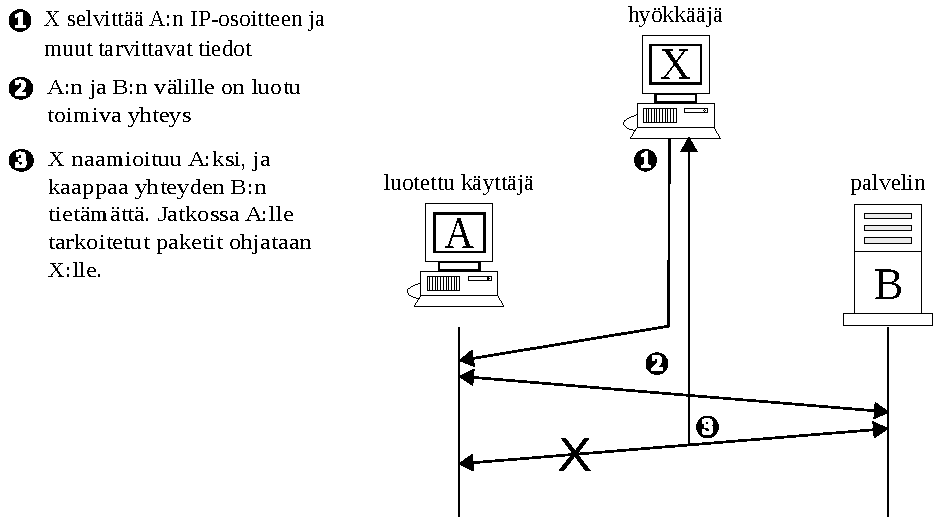
\includegraphics[width=13cm]{pics/MiTM.pdf}
\caption{Man in The Middle-hyökkäys}
\label{Man}
\end{figure}

Vaikka IP-osoitteen väärentämiseen perustuvat hyökkäykset ovat
vaikeita toteuttaa, ovat ne melko yleisiä, sillä jokainen
TCP/IP-protokollaa käyttävä järjestelmä on niille alttiina. Tämä
johtuu siitä, että TCP/IP-verkossa on sallittua muokata paketteja
tiedonsiirron aikana. Näin on, koska eräät IP-pohjaiset palvelut
edellyttävät pakettien sisällön muuttamista lähettämisen
yhteydessä. Tällaisia palveluita ovat esimerkiksi mobiili-IP- ja
VPN-järjestelmät.~\cite{DDOS}.

IP spoofing -hyökkäyksiä voidaan torjua monin eri keinoin. Tehokkain
tapa on määritellä verkon reitittimet estämään sellaisten pakettien
kulku, jotka on merkitty lähetetyiksi sisäverkon laittelta, mutta
jotka todellisuudessa saapuvat reitittimeen sen ulkopuolisista
liitännöistä. Jos tämä kuitenkin halutaan sallia, niin jokainen sessio
tulisi kryptata reitittimessä. Muutenkin yhteyksien muodostumisen
tulisi pohjautua koko järjestelmän kattavaan salaukseen \cite{WEBS}.

% TODO: tarkista, mitä tällä kryptaamisella reitittimessä oikein
% tarkoitetaan.

\subsection{ARP Spoofing}

Nykyisin lähes jokainen verkko pohjautuu TCP/IP-protokollan ja
Ethernet-verkon väliseen yhteistoimintaan. Tässä yhteydessä tarvitaan
ARP-pro\-to\-kol\-laa, jonka tehtävänä on selvittää IP-osoitteita
vastaavat Ethernet- eli MAC-osoiteet. Ethernet-osoite
verkkokorttikohtainen ja sen avulla yksilöidään lähiverkossa
sijaitsevat tietokoneet ja muut aktiivilaitteet.  Tietoa tarvitaan
myös IP-protokollalla liikennöitäessä, koska ilman tietoa
Ethernet-osoitteesta lähiverkossa sijaitseva reititin ei pystyisi
välittämään Internetistä saapuvia paketteja eteenpäin oikealle
laitteelle eikä myöskään lähiverkossa sijaitseva tietokone pystyisi
siirtämään tietoa IP-protokollalla muille lähiverkossa sijaitseville
laitteille.

ARP spoofing -hyökkäyksessä, jota kutsutaan myös ARP-myrkyttämiseksi,
pyritään syöttämään syöttämään reitittimien ARP-tauluihin virheellistä
tietoa (kuva \ref{ARP-spoofing}). Tämä tapahtuu kaappaamalla verkon
yleislähetysviestejä ja muokkaamalla kuittausviestien sisältöä siten,
että kuittausviesteihin hyökkääjä laittaa kohdeosoitteeksi oman
IP-osoitteensa. Verkon aktiivilaitteilta saapuviin, muille
tarkoitettuihin kyselyihin vastataan omalla MAC-osoitteella.  Tämän
jälkeen kohdelaitteelle tarkoitetut paketit ohjautuvatkin hyökkääjän
koneelle \cite{WEBS}.

ARP-protokolla on hyvin haavoittuvainen hyökkäyksille, koska
oletuksena se ei sisällä minkäänlaista suojautumiskeinoa
ARP-myrkyttämiselle. Siksi paras keino suojautua tällaisilta
hyökkäyksiltä on varmistaa, että ennen ARP-taulun muokkausta
tunnistetaan käyttäjät jollakin keinolla. Toinen mahdollisuus on
käyttää verkkolaitteissa staattisia ARP-tauluja~\cite{WEBS}. Jakamalla
lähiverkko pienempiin osiin virtuaalisten lähiverkkojen (VLAN) avulla
voidaan myöskin rajata ARP-myrkyttämisen vaikutuksia.

\begin{figure}[ht]
\centering
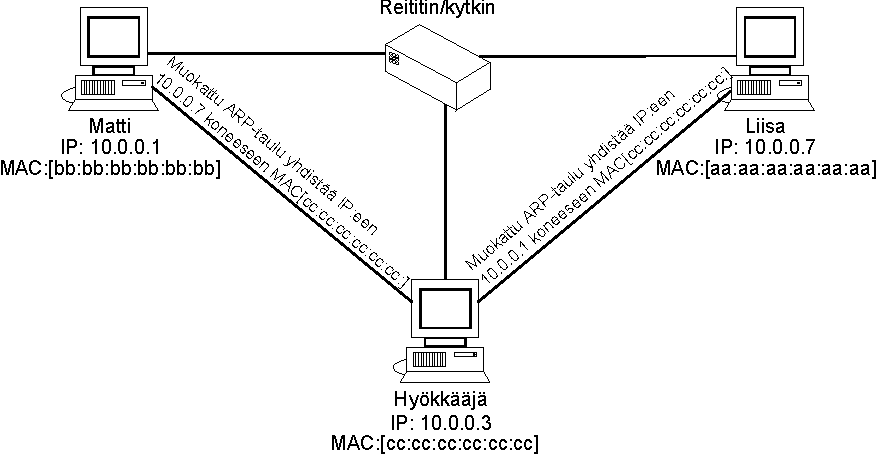
\includegraphics[width=12cm]{pics/arp.pdf}
\caption{ARP-taulun myrkyttäminen käyttäen Man In the Middle -hyökkäystä.}
\label{ARP-spoofing}
\end{figure}

\section{Denial Of Service}

CERT \cite{CERT}, joka on yksi tietoturva-alan johtavista
tutkimuskeskuksista, määrittelee palvelunestohyökkäyksen
(engl. \textit{Denial of Service}, DoS) sellaiseksi teoksi, jossa
hyökkääjän tavoitteena on estää palvelun käyttäjiä käyttämästä heille
kuuluvia tai heidän käytettävissään olevia palveluita. Tällaisia
palveluita voivat olla esimerkiksi tietoliikenneresurssit tai verkossa
käytettävät Web-sovellukset. Hyökkäyksillä pyritään lamauttamaan
palvelua tarjoava verkko tai palvelin siten, että asiaankuuluvien
pyyntöjen vastaanottamiseen tai käsittelyyn ei enää riitä
resursseja. Keinoja hyökkäysten toteuttamiseen on monia. Koska
valtaosa palvelunestohyökkäyksistä käyttää hyväkseen eri protokollien
sallittuja toimintoja, on hyökkäyksiltä suojautuminen hyvin vaikeaa
\cite{Hacking}.

Palvelunestohyökkäykset voidaan jakaa kolmeen ryhmään näiden
toteutustapojen ja tavoitteiden mukaan. Ensimmäiseen ryhmään kuuluvat
hyökkäykset, joiden tarkoituksena on kuormittaa palvelimia ja kuluttaa
loppuun niiden rajoitetut resurssit. Tämä voidaan toteuttaa esimerkiksi
kuormittamalla verkkoa tai palvelinta turhilla pyynnöillä. Toiseen
ryhmään kuuluvat hyökkäykset, jotka pyrkivät joko tuhoamaan tai
muuttamaan konfigurointitietoja siten, että kone tai verkko lakkaa
toimimasta. Viimeiseen ryhmään kuuluvat verkon komponenttien
muokkaamiseen tai tuhoamiseen tähtäävät hyökkäykset
\cite{CERT}. Vaikka tässä työssä keskitytään vain resursseihin
kohdistuviin hyökkäyksiin, niin palvelun kokonaisturvallisuuden
kannalta ylläpitäjän tulee kiinnittää jokaiseen ryhmään tasapuolisesti
huomiota.

% TODO näistä kolmesta voisi tehdä söpön taulukon.

Viime vuosina palvelunestohyökkäysten kirjo on voimakkaasti
laajentunut. Alkuperäisten, pelkästään verkkokerroksen raa’an voiman
hyökkäysten, lisäksi on alkanut esiintyä sovelluskerroksen
hyökkäyksiä, joiden toteuttaminen vaatii hyökkääjältä usein varsin
vähän omia resursseja \cite{Hacking}. Nämä sovelluskerroksen
hyökkäykset ovat toteutukseltaan hyvin hienostuneita, jolloin ne
jäävät yleensä huomaamatta tavanomaisilta tietoturvajärjestelmiltä,
koska tietoliikenteen sisältö ei juurikaan poikkea
normaalitilanteesta. Hyökkääjä saattaa esimerkiksi pyytää sellaista
resurssia palvelulta, jonka kysely vie vain vähän hyökkääjän omia
resursseja, mutta aiheuttaa palvelimelle suuren kuormituksen
\cite{DDOSb}.

Sovelluskerroksen hyökkäysten teho nähtiin vuonna 2004, kun
MyDoom-\-viruksella saastuneet koneet kuormittivat yleisimpiä
hakukoneita etsimällä näiden avulla uusia sähköpostiosoitteita, joihin
lähettää saastunut sähköposti \cite{Hacking}. Sovelluskerroksen
hyökkäyksen vaikutus voidaan kohdistaa myös yksittäisiä palveluita
kohti, jolloin vaikutukset ovat vieläkin suuremmat. Näin tapahtui
vuonna 2003, kun Yhdysvalloissa yrittäjä palkkasi ns. DDoS-mafian
kaatamaan kilpailijoidensa verkkosivut HTTP-kyselyillä, jotka pyysivät
ladattavaksi isoa kuvatiedostoa \cite{DDOSb}. Tämä aiheutti kolmelle
kilpailijalle arviolta jopa miljoonan dollarin tappiot ja pysäytti
näiden liiketoiminnan lähes kahdeksi viikoksi \cite{FBI}.

\subsection{SYN-hukuttaminen}
TCP/IP-protokollan yksi suunnittelulähtökodista oli, että sitä
käytettäisiin avoimessa ja luotetussa ympäristössä. Tästä syystä sen
suunnittelussa ei osattu ottaa huomioon mahdollisia vihamielisiä
käyttäjiä, jotka pyrkisivät häiritsemään muiden käyttäjien
tietoliikennettä. TCP/IP-protokollan käyttö julkisissa verkoissa kuitenkin
yleistyi arvaamattomasti, jonka vuoksi suunnitteluvaiheessa tehdyt
virheet periytyivät nyt käytössä olevaan IPv4-verkkojen rakenteisiin
\cite{Hacking}.

Yhteydenmuodostus TCP-protokolla tapahtuu kolmivaiheisesti. Aluksi
yhdistävä tietokone lähettää palvelimelle SYN-paketin, jonka
seurauksana palvelin varaa tulevalle yhteydelle resursseja ja lähettää
yhdistävälle tietokoneelle SYN/ACK-paketin. Tämän jälkeen palvelin
jää odottamaan yhteyden muodostamista. Tähän yhdistävän tietokoneen
tulee vastata ACK-paketilla, jonka jälkeen yhteys on muodostunut ja
tiedonsiirto voi alkaa \cite{Hacking}. Tunnetuin TCP:tä käyttävä
protokolla on Webissä käytettävä HTTP. Sen avulla Web-palvelimet
pystyvät nopeasti palvelemaan useita yhtäaikaisia käyttäjiä.

TCP/IP-protokollan historiasta perityistä heikkouksista tunnetuin ja
käytetyin on SYN-hukuttamiseksi kutsuttu hyökkäys, jossa hyökkääjä
pyrkii kuluttamaan kohteen tietoliikennekapasiteetin loppuun
tekaistuilla yhteydenmuodostuspyynnöillä. Hyökkäys on hyvin
yksinkertainen ja helppo toteuttaa, sillä se käyttää hyväkseen
TCP-protokollaan määritettyjä toimintoja. Hyökkäyksessä
TCP-protokollan kolmiosaista yhteydenmuodostusta ei viedä loppuun
saakka vaan jätetään palvelin odottamaan ACK-paketti yhdistävältä
tietokoneelta.

Koska TCP-protokolla pyrkii aina varmistamaan yhteyden muodostumisen,
lähetetään SYN/ACK-paketti tarvittaessa uudestaan, kunnes yhdistävä
tietokone vastaa ACK-paketilla tai määritelty aikaraja tulee
vastaan. Tätä ominaisuutta hyökkääjä pystyy käyttämään
hyväkseen. Riittää, että hyökkääjä nuuskii selville käyttämättömän
IP-osoitteen, joka on vielä mieluiten samasta aliverkosta kuin missä
palvelin sijaitsee. Tämän jälkeen hyökkääjä luo SYN-paketin, jossa on
tämä tekaistu IP-osoite. Koska palvelimen lähettämä SYN/ACK-viesti ei
koskaan saavu oikealla koneelle, ei palvelin saa ACK-kuittausta. Tällöin
TCP-protokolla alkaa lähettämään pakettia uudestaan niin kauan
kunnes määritetty raja yhteyden aikakatkaisulle tulee vastaan
\cite{STACK}. Hyökkääjän on vaivatonta automatisoida nämä vaiheet ja
hyökkäys voidaan toteuttaa esimerkiksi saastuneista koneista
muodostetun verkoston avulla. Näin saadaan aikaiseksi kuvan \ref{syn}
mukainen tilanne, jossa useita IP-osoitteita käyttämällä hyökkääjä
häiritsee kohteen toimintaa turhilla yhteydenottopyynnöillä.

\begin{figure}[hpt]
\centering
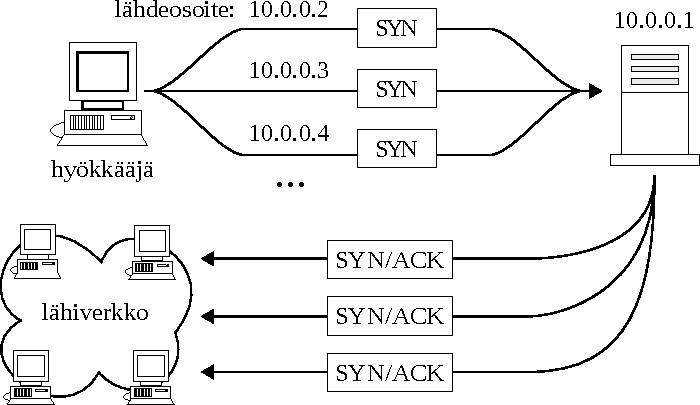
\includegraphics[width=12cm]{pics/syn.pdf}
\caption{SYN-hyökkäys käyttäen useita lähiverkon IP-osoitteita.}
\label{syn}
\end{figure}

SYN-hukuttamisen mahdollistavan mekanismin avulla voidaan myös toteuttaa
heijastettu hyökkäys (engl. \textit{reflective attack}), joka on muunnos 
SYN-hukuttamisesta. Tässä hyökkäyksessä väärennetyissä SYN-viesteissä on
lähettäjäksi merkitty haluttu kohde. Lähettämällä suuri määrä näitä SYN-viestejä 
esimerkiksi Web-\-palvelimelle, aiheutuu vastaustulvasta ongelmia
kohteelle \cite{STACK}.

Koska ylimääräistä palvelinkapasiteettia ei useinkaan ole järkevää
pitää SYN-\-hukuttamisen varalta, joudutaan ratkaisua
hakemaan muualta. Alkeellisin keino on rajoittaa puoliavonaisten
yhteyksien määrää, jolloin rajan ylittyessä yhteyksiä aletaan
pudottamaan \cite{TCP}. Toinen käytetty keino on reitittimiltä
verkkoon päin tulevan liikennemäärän seuraaminen ja liikennepiikkeihin
reagoiminen. Hyökkäyksiä vastaan voidaan myös suojautua liikenteen
seuraamiseen tarkoitetuilla sovelluksilla sekä pääsylistoilla
\cite{STACK}.

Kehittyneempi suojautumiskeino on muuttaa TCP-protokollan kättelyä
siten, että yhteyden tarvitsemat resurssit varataan vasta ACK-viestin
vastaanottamisen yhteydessä. Tätä menetelmää kutsutaan
SYN-evästykseksi (engl. \textit{SYN Cookies}) ja se on tuettu
mm. Linuxissa ja FreeBSD:ssä~\cite{syncookies}. Yhteydenmuodostuksessa
tarvittavat parametrit kätketään tällöin SYN-paketin
järjestysnumeroon. Tämän menetelmän käyttö kuitenkin rajaa pois
runsaasti TCP-protokollan ominaisuuksista, jonka vuoksi SYN-evästys
kytketään yleensä päälle vain hyökkäysten ajaksi.

Täydellistä ratkaisua SYN-hukuttamista vastaan ei mikään näistä
tavoista kuitenkaan tarjoa. Huolellisesti toteutettua hyökkäystä on
vaikea torjua.

\subsection{UDP Echo}

Myös UDP-protokollan käyttö mahdollistaa hyökkäysten tekemisen. Nämä
hyökkäykset käyttävät hyväkseen UDP Echo -protokollaa, mikäli sen
käyttö on sallittu verkossa. Näistä hyökkäyksistä tunnetuin on
Fraggleksi nimetty hyökkäys, joka nykyisinkin aiheuttaa väärin
konfiguroidussa verkossa suuria ongelmia.  Fraggle toimii siten, että
hyökkääjä lähettää UDP Echo -viestin yleislähetyksenä, johon on
merkitty lähettäjäksi hyökkäyksen kohde. Tähän viestiin kaikki verkon
koneet pyrkivät vastaamaan, jolloin kohdetietokoneen
tietoliikennekapasiteetti ja resurssit käytetään viestien
vastaanottamiseen (kuva \ref{fraggle}).

Fraggle on hyvä esimerkki vahvistetusta hyökkäyksestä, jossa verkon
laitteiden määrä vaikuttaa siihen, kuinka vakava hyökkäys on
\cite{WEBS}. Vastaavanlainen hyökkäys voidaan myös toteuttaa kahden
koneen välillä, jos kummassakin on sallittuna UDP Echo
-viestit. Tällöin hyökkääjä väärentää viestiin lähettäjän osoitteen ja
halutun kohdeportin. Vastaanottaja vastaa tähän viestiin omalla
Echo-viestillä, ja näin kahden koneen välille muodostuu ikuinen
silmukka \cite{TCP}.

\begin{figure}[htp]
\centering
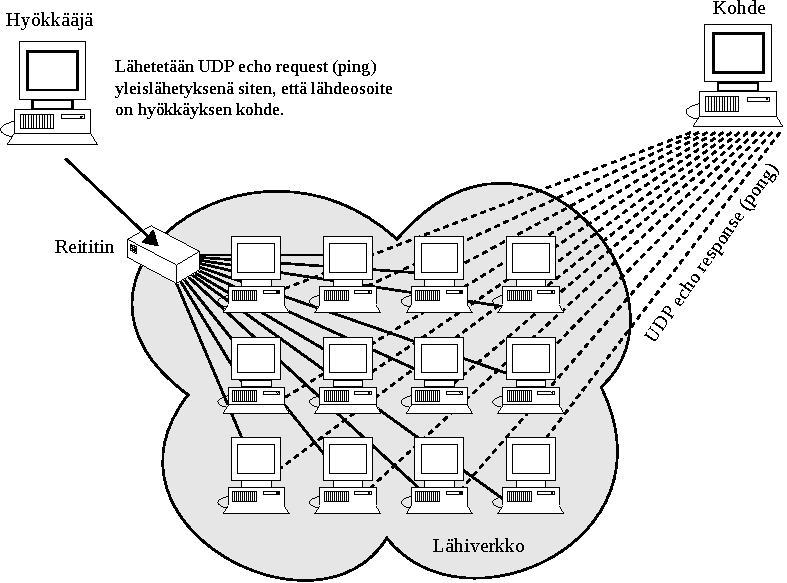
\includegraphics[width=13cm]{pics/fraggle.pdf}
\caption{Vahvistettu UDP Echo -hyökkäys.}
\label{fraggle}
\end{figure}

\subsection{Smurf}

Smurf on yksi ensimmäisistä vahvistetuista DoS-hyökkäyksistä, ja se
toimii lähes identtisesti Fragglen kanssa sillä erolla, että UDP:n
sijasta käytetään ICMP-\-protokollaa. Hyökkääjä lähettää kohteen
puolesta yleislähetyksenä verkolle ICMP Echo -paketin, johon verkon
laitteet vastaavat, jos Echo-viestit on sallittuja verkossa. Jo 100
tietokoneen lähiverkko pystyy aiheuttamaan 14 Mb/s haittaliikenteen
kohdekoneelle, joten pienessäkin väärin konfiguroidussa verkossa
on mahdollista muodostaa riittävästi haittaliikennettä tietoliikenteen
häiritsemiseen tai estämiseen \cite{Hacking}.

Jos hyökkäys on päässyt käyntiin, ei tälle ole paljoa muuta tehtävissä
kuin poistaa kohteena olevat laitteet pois verkosta. Paras vastatoimi
Fragglen ja Smurffin kaltaisille hyökkäyksille on konfiguroida verkon
laitteet alusta asti oikein. ICMP Echo -yleislähetysten estämisellä
pääsee jo pitkälle. ICMP-protokollan käyttöä verkossa kannattaa
muutenkin tarkkailla ja tarvittaessa rajoittaa \cite{Hacking}.

\section{Distributed Denial of Service}

Vielä viime vuosikymmenellä palvelunestohyökkäykset perustuivat
yleensä käyttöjärjestelmistä löydettyjen heikkouksien
hyödyntämiseen. Näiden hyökkäysten aikaansaama tuho riippui paljon
käytettävistä järjestelmistä ja vahingot olivat melko
rajattua. Palvelunestohyökkäyksiä ei nähty tällöin kovinkaan vakavana
uhkana, mutta suhtautuminen muuttui 2000-luvulle tultaessa, kun
hajautetut palvelunestohyökkäykset (engl. \textit{Distributed Denial
of Service}) kehitettiin. Tällaisessa hyökkäyksessä palvelua saattaa
olla lamauttamassa jopa yli 140~000 saastunutta konetta. Tällaisia
saastuneita koneita kutsutaan zombeiksi (engl. \textit{zombie}).

Tietokone voidaan muuttaa zombiksi murtautumalla ja asentamalla siihen
ohjelmisto, jonka avulla murtautuja pystyy hallitsemaan laitetta
käyttäjän tietämättä. Zombiverkoston ei tarvitse edes olla kovinkaan
suuri aiheuttaakseen tuhoa, sillä jo 3~000 koneen verkosto, jossa
jokainen kone tuottaa 25 kb/s liikennettä, aiheuttaa yhteensä 75 Mb/s
kuormituksen verkolle \cite{Hacking}.  Palvelunestohyökkäyksen
seuraamukset ovat varautumattomalle taholle usein katastrofaaliset ja
pahimmillaan hyökkäys saattaa pysäyttää organisaation toiminnan
useiksi päiviksi \cite{CERT}.

Hyökkäysten hajauttaminen useammalla koneelle tuo useita hyötyjä
verrattuna perinteiseen palvelunestohyökkäykseen, jossa hyökkäys
toteutetaan käyttäen yhtä konetta. Otetaan esimerkiksi vaikka
Web-palveluita tarjoava palvelin, jota vastaan halutaan tehdä
palvelunestohyökkäys. Tällaisella palvelimella on käytössä
huomattavasti suurempi määrä resursseja (tietoliikennekapasiteetti,
muisti, laskentateho) kuin yksittäisellä zombitietokoneella on. Kun
hyökkäys suoritetaan yhtäaikaisesti useammalla koneella, pystyy
hyökkääjä kuluttamaan suuretkin resurssit loppuun lyhyessä
ajassa. Yksittäiseltä koneelta tuleva palvelunestohyökkäys on helppo
tunnistaa ja estää verkon ylläpitäjän toimesta. Hyökkääjien määrän
kasvaessa tehtävä vaikeutuu huomattavasti, koska haittaliikennettä
aiheuttavat tietokoneet tai itse haittaliikenne pitää tunnistaa
hyötyliikenteen joukosta. Mikäli zombitietokoneet ovat sijoittuneet ympäri
Internetiä, on hyökkäysten pysäyttäminen ilman palvelun laadun heikkenemistä
mahdoton tehtävä ilman automatisointia. Haittaliikennettä on tällöin myös
vaikea erottaa tavallisesta liikenteestä, koska se tulee palvelimelle
useita reittejä pitkin \cite{DDOS}.

Nopeiden yhteyksien ja verkossa olevien tietokoneiden räjähdysmäinen
kasvu on tehnyt hajautetuista palvelunestohyökkäyksistä hyvin
tehokkaita ja tuhoisia. Suuri määrä verkkoon liitetyistä laitteista on
huonosti suojattu ja päivitetty, ja ihmisten tietoisuus verkon
vaaroista on usein puutteellista. Tämä on luonut otollisen maaperän
suurten zombiverkostojen muodostamiselle virusten ja matojen
avustuksella. Tarjolla on myös tätä tarkoitusta varten suunniteltuja
työkaluja ja ohjelmistoja, jotka tekevät tarvittavat toimenpiteet
automaattisesti. Jo ensimmäiset, vapaasti saatavilla olevat työkalut,
kuten Trinoo ja Shaft, mahdollistivat tuhansien suojaamattomien
koneiden haltuunoton ilman suurempaa perehtymistä \cite{DDOS}.

Hyökkäyksessä käytetyt koneet voidaan jakaa agentteihin (engl. \textit{agents})
ja liikenteen ohjaajiin (engl. \textit{handlers}) riippuen näiden
rooleista. Näistä koneista hyökkääjä käskyttää suoraan liikenteen
ohjaajia, jotka ohjaavat edelleen annetut käskyt agenteille
hyökkäyksen alettua \cite{WEBS}\cite{DDOS}. Ensimmäisissä 
DDoS-verkoissa nämä ohjausviestit olivat salaamattomia, jolloin kuka tahansa
pystyi kaappaamaan näitä. Tämä oli tietomurtojen tekijöiden
näkökulmasta ongelmallista, koska liikenteen ohjaajat joutuivat
ylläpitämään listaa agenttien käyttämistä IP-osoitteista. Mikäli liikenteen välittäjä
joutui vastahyökkäyksen kohteeksi, pystyttiin selvittämään zombiverkon jokaisen
laitteen osoitteet. Tätä suoran käskyttämisen heikkoutta pyrittiin korjaamaan muun
muassa salaamalla käytettävä viestiliikenne. Ajan saatossa liikenteen
ohjaajat pystyttiin kuitenkin tunnistamaan ja poistamaan verkosta,
jolloin hyökkäyksessä käytetty zombiverkko hajosi \cite{DDOS}.

\begin{figure}[htp]
\centering
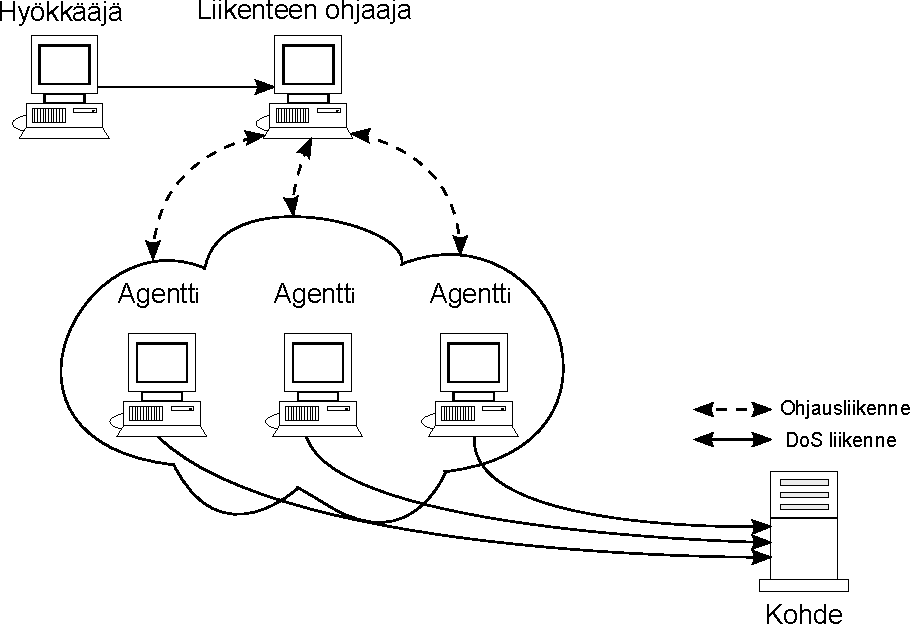
\includegraphics[width=12cm]{pics/perinteinen_ddos.pdf}
\caption{Perinteinen DDoS-verkosto}
\label{ddos1}
\end{figure}

Nykyisin enää harva DDoS-hyökkäyksessä käytetty verkko käyttää kuvan
\ref{ddos1} hierarkiaa sen heikon ohjattavuuden takia. Tämän tilalle
on tullut epäsuoraan käskyttämiseen perustuvat verkot, jotka käyttävät
viestien välittämiseen IRC-verkkoja (kuva \ref{ddos2}). IRC on
reaaliaikaiseen viestittämiseen tarkoitettu palvelu, jonka kautta
ihmiset pystyvät reaaliajassa kirjoittamaan ja lukemaan
viestejä. IRC-verkot koostuvat käyttäjistä ja IRC-kanavista, joille
käyttäjät voivat halutessana liittyä. Epäsuoran käskyttämisen
periaatteella toimivat verkot hyödyntävät näitä samoja
ominaisuuksia. Jokainen kone liittyy IRC-kanavalle, joka on yleensä
salasanalla suojattu. Kanavan kautta hyökkääjä voi antaa käskyjä
koneille. Tällä tavalla saadaan monia etuja verrattaessa suoraan
käskyttämiseen.  Ensinnäkin liikennettä ei pystytä enää tunnistamaan
poikkeavaksi, koska se on tavanomaista IRC-liikennettä. Toisekseen
käytettyä kanavaa voidaan vaihtaa lennosta, jolloin yhden kanavan
sulkeminen ei pysäytä verkon toimintaa. Näiden syiden takia
DDoS-hyökkäysten pysäyttäminen ennen niiden käynnistymistä on erittäin
vaikeaa \cite{DDOS}.

\begin{figure}[t]
\centering
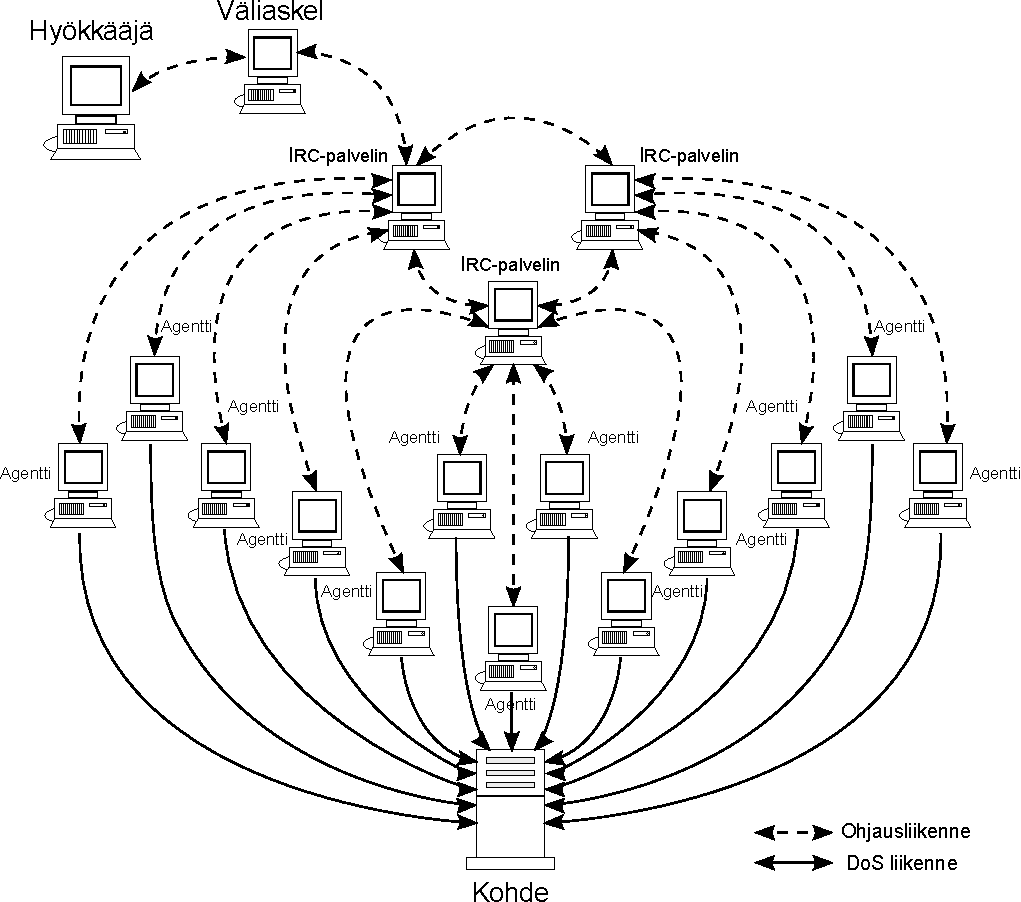
\includegraphics[width=12cm]{pics/ddos_uusi.pdf}
\caption{Nykyisin käytetty DDoS-verkosto}
\label{ddos2}
\end{figure}

% FIXME: Mitä hittoa seuraava kappale tarkoittaa?

Kuten yllä on jo tullut esille, on hajautetulta palvelunestohyökkäykseltä
suojautuminen vaikea tehtävä riippumatta siitä, onko verkko itse kohde vai
käytetäänkö sitä vain hyökkäysten koordinointiin. Valmista ja yksityiskohtaista
ratkaisua ei ole tarjolla, mutta seuraamalla joitakin yleisiä strategioita,
voidaan vahinkoja rajoittaa. Nämä strategiat ovat suojautuminen, tunnistaminen
ja reagoiminen, ja ne noudattavat vahinkoketjun yleistä elinkaarta \cite{DDOS}.

% FIXME: Pitäisikö tämä muutenkin siirtää jonnekin muualle, ei liity
% DDOSiin vaan tietoturvastrategioihin yleensä.

Ensinnäkin on tärkeää, että verkon ylläpitäjä tietää tarkoin kuinka verkko
toimii ja hyödynnetään verkon toimintaa analysoivia työkaluja. Näiden avulla
verkon heikot kohdat pystytään tunnistamaan ja vahvistamaan. Käytössä tulee
olla myös jonkinlainen suojausjärjestelmä, joka kirjaa ylös riittävän pitkältä
ajalta ylös verkkoon tulevan ja lähtevän liikenteen, sillä aina hajautettu
palvelunestohyökkäys ei kaada koko verkkoa. Tällöin on tärkeää, että tapahtunut
pystytään tarkasti analysoimaan ja löydetyt heikkoudet paikattua parhaalla
mahdollisella tavalla \cite{DDOS}.

Kun hyökkäys on meneillään, tulee käytetty hyökkäystapa tunnistaa mahdollisimman
nopeasti. Useimmat hyökkäykset noudattavat tiettyä kaavaa, ja näiden
tunnistamiseen on olemassa useita valmiita työkaluja. Tämä on tärkeää, koska
tunnistamisen jälkeen voidaan rajata, mistä hyökkäys on peräisin ja tehdä
tarvittavat toimenpiteet hyökkäyksen torjumiseksi. Useimmissa tapauksissa
tämä tarkoittaa yhteistyötä palveluntarjoajan ja viranomaisten kanssa.
Viranomaisten mukaan tuominen on muutenkin tärkeää, koska vain tätä kautta
voidaan käytettyä hyökkäysverkostoa lähteä tunnistamaan ja toivottavasti myös
hajottamaan \cite{DDOS}.

Jotta nopea reagoiminen olisi mahdollista, tulee organisaatiolla olla
toimintasuunnitelma hyökkäyksen varalta. Ensimmäinen vaihtoehto lienee aina
haitallisen liikenteen estäminen, mutta tätä varten tulee olla tehtynä tarkat
prosessit kuinka toimitaan hyökkäyksen alettua. Tärkeää on sopia mitä
dokumentoidaan ja kuinka asioista raportoidaan oikeille tahoille. Hyökkäyksen
jälkeinen analyysi on myös riippuvainen sovituista käytännöistä. Tämä analyysi
on erittäin tärkeää, sillä vain sitä kautta toimintasuunnitelmia voidaan
kehittää oikeaan suuntaan \cite{DDOS}.


\section{Remote-to-Local}

Remote-to-Local (lyh. \textit{R2L}) on hyökkäystyyppi, jossa hyökkääjä pyrkii
saamaan koneelle laajemmat oikeudet, kuin hänellä muuten
olisi. Tämä tapahtuu useimmiten käyttäen hyväksi järjestelmässä olevia
heikkouksia, joiden avulla hyökkääjä pääsee verkon yli murtautumaan
koneelle \cite{IDS}. Pahimmassa tapauksessa hyökkääjä saa hankittua koneelle
pääkäyttäjän oikeudet, jolloin koneen ja verkon resurssit ovat täysin
hyökkääjän käytettävissä.

Onnistuneet R2L-hyökkäykset ovat verkon ylläpitäjien kannalta pahimpia
mahdollisia, sillä niiden mahdollistamat tuhot ja aiheuttamat kustannukset ovat
huomattavasti suurempia verrattuna muihin hyökkäystyyppeihin \cite{IDSb}. Onnistunut R2L-hyökkäys saattaa
myös muut lähiverkon koneet vaaraan, sillä usein hyökkääjä pyrkii asentamaan
koneisiin ohjelmistoja, joiden avulla hyökkääjä pystyy ottamaan koneen haltuun
käyttäjän huomaamatta. Tällä tavoin osa aikaisemmin mainituista
zombverkostoista saa alkunsa.

Käytetyimmät Web-palvelinohjelmistot, Apache ja IIS, vastaavat noin 85~\%
kaikista käytetyistä palvelinsovelluksista. Näiden kahden lisäksi
BIND-\-ohjelmistoa käytetään valtaosassa nimipalvelimista. Ohjelmistojen yleisyydestä
johtuen yli puolet R2L-hyökkäyksen mahdollistavista heikkouksista onkin
löydetty näille alustoille \cite{IDS}. Useat haavoittuvaisuudet johtuvat
ohjelmointivirheistä, joiden johdosta hyökkääjä pystyy aiheuttamaan
sovellukseen muistin ylivuodon (engl. \textit{Buffer Overflow}). Tämä usein kaataa
sovelluksen tai saattaa sen sellaiseen tilaan, jossa hyökkääjä pystyy ajamaan
omia komentoja koneella. Kattava listaus löydetyistä haavoittuvuuksista ja näiden
korjauksista löytyy osoitteesta \url{www.cve.mitre.org/cve} \cite{CVE}.

Tunnetuilta R2L-hyökkäyksiltä suojautuminen on hyvin yksinkertaista, sillä
nykyinen trendi on, että haavoittuvuuden löytänyt taho ilmoittaa siitä
yleensä ensin
sovelluksen kehittäjille ennen julkista ilmoitusta. Siksi korjaus
haavoittuvuuteen on usein olemassa ennen kuin sitä on mahdollista hyödyntää \cite{IDSb}.
Vastuu jääkin verkon ylläpitäjälle, että käytetyt sovellukset ja 
suojausjärjestelmät pidetään ajan tasalla, sillä suurin osa onnistuneista hyökkäyksistä 
johtuu siitä, että tunnettuja tietoturva-aukkoja ei ole korjattu.

\section{User-to-Root}

User-to-Root (lyh. \textit{U2R}) hyökkäyksessä murtautuja pyrkii hankkimaan
koneelle pääkäyttäjän oikeudet. Tämä tapahtuu käyttäen järjestelmässä
olevia haavoittuvaisuuksia, joita ei ole paikattu. Useimmiten
hyökkäykset pohjautuvat koodausvirheisiin, jotka mahdollistavat
ylivuodon aiheuttamisen sekä odottamattomien syötteiden antamisen
\cite{IDS}. Käyttäjästä pääkäyttäjäksi hyökkäys eroaa R2L hyökkäyksestä
siten, että hyökkääjällä on jo valmiiksi pääsy koneelle tavallisen
käyttäjän oikeuksilla.

U2R-hyökkäykset ovat L2R-hyökkäysten ohella vaikeimpia torjua, jos kohteena
oleva järjestelmä on altis U2R-hyökkäyksille. Vaikea torjuttavuus johtuu siitä, että
usein hyökkäyksestä aiheutuva liikenne muistuttaa hyvin paljon normaalia
liikennettä, jonka vuoksi itsestään oppivat puolustusjärjestelmät eivät pysty
riittävän tarkasti erottamaan haitallista liikennettä normaalista \cite{U2R}.
Kehittyneimmilläkin järjestelmillä näiden hyökkäysten tunnistaminen on todella
heikkoa. Tämän on osoittanut useat eri tutkimushankkeet, jotka ovat käyttäneet
järjestelmiensä testaamiseen DARPAn simuloimaa verkkoliikennettä,
jossa olevat tietomurrot ja muu poikkeava toiminta on merkitty.
Parhaimmillaankin tunnistaminen on jäänyt 20 prosentin
paikkeille.

% -*- mode: LaTeX; coding: utf-8; -*-

\chapter{Hyökkäysten torjunta ja ennustaminen}

\todo{Tarvitaanko tätä ollenkaan? Otetaanko pois vai laitetaanko
jotakin tilalle?}

TODO.

% -*- mode: LaTeX; coding: utf-8; -*-

\chapter{Aiheeseen liittyvä tutkimus}

\section{Yleistä}

Viime vuosina web-sovellukset ovat kasvattaneet suuresti suosiota, ja nykyisin yhä useampi palvelu, jossa tietoturvan ja saatavuuden takaaminen on elintärkeää, on siirtynyt osittain tai kokonaan 
verkon puolelle. Tämä on vaikuttanut suuresti siihen, mihin tietoturvahyökkäykset nykyisin kohdistuvat, ja kuinka niitä pyritään toteuttamaan. Hyökkäysten muuttuessa yhä hienostuneimmiksi, 
eivät perinteiset tietoturvamenetelmät enää riitä suojaamaan loppukäyttäjiä tai palvelun ylläpitäjiä. Tästä syystä erilaisten tietoturvaratkaisuiden ympärillä käy kova kuhina, ja aihepiiri 
on herättänyt suurta kiinnostusta tutkijoiden keskuudessa. Erilaisia ratkaisuja, joissa on pyritty selvittämään aikaisemmissa luvuissa esitettyjä tietoturvahyökkäyksiä ja näiden 
mukana tulleita haasteita, on lukematon määrä. Seuraavaksi esitellyt tutkimukset edustavat vain pientä osaa koko tutkimuskentästä, mutta jo näistä käy ilmi se, millaisia ratkaisumalleja
nykyisin etsitään.

Hyökkäysten tunnistaminen toimii siten, että analysoimalla yhtä tai useampaa tapahtumaa pyritään löytämään viitteitä tapahtuvista hyökkäyksistä. Tunnistamiseen pohjautuvat menetelmät jaetaan usein
kahteen eri tyyppiin: anomalioiden eli poikkeavuuksien tunnistamiseen (eng. anomaly detection) ja väärinkäytösten tunnistamiseen (eng. misuse detection). Näistä anomalioiden tunnistamiseen perustuvat
järjestelmät luovat malleja järjestelmän, käyttäjän tai verkon normaalista käyttäytymisestä, ja vertaamalla tapahtumia näin muodostettuihin kuvauksiin, voidaan poikkeavuudet tunnistaa. Väärinkäytösten 
tunnistamiseen tarkoitetut järjestelmät taas sisältävät joukon kuvauksia eli signatuureja tunnetuista hyökkäyksistä. Tuleva liikenne tarkistetaan näitä kuvauksia vastaan, jolloin kuvauksia vastaavat
hyökkäykset voidaan tunnistaa. Joissakin tapauksissa jaottelu on myös tehty sen mukaan, mistä tutkittava liikenne on kerätty. Tällöin järjestelmät on jaettu verkkoon pohjautuviksi (eng. network based)
ja asiakaspohjaisiksi (eng. host based). 

\section{Väärinkäytösten tunnistaminen}

Väärinkäytökseen perustuvat järjestelmät ovat pitkään olleet suosituin lähestymistapa hyökkäysten torjumiseen. Nämä järjestelmät on voitu jakaa kahteen erilliseen osaan, jossa tilattomassa 
järjestelmässä jokaista tulevaa tapahtumaa käsitellään itsenäisesti, kun taas tilallisessa järjestelmässä tutkitaan tapahtumien välisiä suhteita. Web-pohjaisten hyökkäysten tutkimisessa tietolähteinä 
on käytetty mm. palvelimien tuottamaa lokia \cite{LightTool}, ja IDS-järjestelmien \cite{Snort}\cite{Bro} tapauksessa analysoimalla verkkokerroksen liikennettä. Ensimmäisessä ratkaisussa ongelmana
on, että itse palvelimiin kohdistuvia hyökkäyksiä ei pystytä havaitsemaan ainoastaan lokitietoa tarkkailemalla. Samoin hyökkäyksiä, jotka koostuvat monista eri vaiheesta, on mahdotonta mallintaa. 
Verkkokerroksella toimivia järjestelmiä taas pystytään harhauttamaan muokkaamalla hyökkäyksiä, ja näistä harvat mahdollistavat tilallisen analyysin. 

Esitettyjä ongelmia on pyritty ratkaisemaan lisäämällä havaittavien tapahtumien määrää, ja keräämällä informaatiota eri lähteistä. Esimerkiksi asentamalla sovellustasolle erillinen tiedonkeruuseen 
tarkoitettu komponentti \cite{Application} on saatu hyviä tuloksia. Tässä tapauksessa tiedonkeruu tapahtui Apache-palvelimelle asennetun komponentin välityksellä, joka tarkkaile lokitiedon lisäksi
mm. pyyntöjen tulkitsemiseen ja toteuttamiseen menevää aikaa. Tämän ratkaisun etuna on myös se, että tutkittava data on salaamattomassa muodossa, ja sessioiden uudelleenrakentaminen on mahdollista. 
Tällä tasolla toimiva IDS-järjestelmä voi myös toimia ennaltaehkäisevästi eli haitalliseksi havaittu liikenne voidaan tiputtaa pois ennen kuin se käsitellään palvelimella. Suurimpana haittapuolena on, 
että tietylle sovellukselle suunniteltua komponenttia ei voida sellaisenaan käyttää muilla alustoilla. 

WebSTAT \cite{Webstat} on tilalliseen analyysiin perustuva IDS-järjestelmä, joka pohjautuu STAT-kehitysympäristöön \cite{STAT}. WebSTAT hyödyntää STATL-ohjelmointikieltä, joka mahdollistaa hyökkäysten
mallintamisen ottamalla huomioon mm. eri tapahtumien välisiä yhteyksiä ja verkkohistoriaa sekä palvelimien kuten Apachen ja Microsoftin IIS:n lokia. Koska tietoa kerätään yhtäaikaisesti monesta eri 
lähteestä, voidaan palvelimien lokitiedon analysointiin yhdistää alempien toimintojen kuten jär\-jes\-tel\-mä- ja verkkotason tuottamaa tietoa. Näin tehty analyysi kuvaa koko järjestelmä tilaa, jolloin 
yllättävät muutokset pystytään havaitsemaan nopeasti. Testien mukaan tällainen analyysi voidaan toteuttaa suurissa järjestelmissä reaaliajassa aiheuttamatta suurempaa viivettä palvelimien toiminnassa. 
Menetelmän sovittaminen tiettyyn järjestelmään vaatii jonkin verran manuaalista työtä, ja tätä voidaankin pitää sen suurimpana heikkoutena. Monimutkaisten hyökkäysten kuvaaminen on usein myös hankala
toteuttaa, ja niiden tulkitsemiseen saattaa tuhlaantua turhaa aikaa.

Väärinkäytösten tunnistamiseen tarkoitettuja järjestelmiä on hyödynnetty myös uudempien tietoturvahyökkäysten tunnistamisessa. Esimerkiksi vihamielisten Flash-mainosten tunnistamiseen tarkoitettu 
OdoSwiff \cite{FlashAdd} pyrkii etsimään sivuilla olevista mainoksista hyökkäykseen tarkoitettua koodia käyttäen staattista ja dynaamista analyysia. Palvelinpuolella XSS-hyökkäyksiä vastaan on luotu 
järjestelmä, josta löytyy yleisimpien hyökkäysten kuvaukset \cite{SignatureXSS}. Kumpikin järjestelmistä toimii erittäin hyvin, kunhan hyökkäys on entuudestaan tuttu.

\section{Poikkeavuuksien tunnistaminen}

Väärinkäytösten tunnistamiseen käytettyjen järjestelmien suurin heikkous piilee siinä, että mallintamattomat hyökkäykset jäävät näiltä huomaamatta. Tämä on erityisesti web-palveluihin kohdistuvien
hyökkäysten tapauksessa iso ongelma, sillä toimintaympäristö muuttuu jatkuvasti, ja uusia hyökkäyksiä ja vanhojena variaatioita ilmestyy tiuhaan tahtiin. Tällöin signatuurien pitäminen ajantasalla
muodostuu mahdottomaksi tehtäväksi. Hyökkäysten monimuotoisuus onkin johtanut siihen, että nykyisin yhä useammassa järjestelmässä pyritään tunnistamaan poikkeavat tapahtumat normaaliin liikenteen seasta
ilman tarkkoja signatuureja. 

Anomalioiden tunnistamiseen on käytössä useita eri menetelmiä, ja ne voidaan jakaa kahteen eri ryhmään \cite{State}. Näistä ensimmäinen sisältää oppimiseen pohjautuvat mallit, jossa normaali 
käyttäytyminen opetetaan opetusmateriaalin avulla. Normaalia käyttäytymistä esittävät profiilit voidaan mallintaa käyttäen joko sään\-tö\-poh\-jais\-ta-, mallipohjaista- tai tilastopohjaista menetelmää. Näistä
sääntöpohjaiset menetelmät muistuttavat eniten perinteisiä IDS-järjestelmiä sillä erolla, että luodut säännöt pohjautuvat kerättävään dataan, ja säännöt voivat olla rakenteiltaan hyvin monimutkaisia. 
Mallipohjaisissa menetelmissä taas luodaan normaalia käyttäytymistä kuvaavat profiilit, jota vastaan tuleva liikenne arvioidaan. Tiedonlouhinta, neuroverkot ja liikenteestä luotujen kuvioiden vertaaminen
tulevaan liikenteeseen (eng. pattern matching) ovat tekniikoita, joita on käytetty tällaisten mallien luomiseen. Analyysissa voidaan esimerkiksi tutkia verkkopakettien kuormia \cite{Payload}\cite{ULISSE} 
ja klusteroimalla ja luokittelemalla liikenne protokollien ja palveluiden mukaan \cite{Cluster}. Viimeisen ryhmän muodostavat tilastollisiin menetelmiin pohjautuvat menetelmät \cite{PacketHeader}, jotka
ovat jääneet vähemmälle huomiolle johtuen alati muuttuvasta toimintaympäristöstä.

Toisen ryhmä anomalioiden tutkimisessa muodostavat spesifistiset mallit (eng. spesification model). Nämä menetelmät pohjautuvat enemmän ihmisten huomioihin ja asiantuntijuuteen kuin matemaattisiin
kuvauksiin. Menetelmissä käytetään useita eri elementtejä aina sovellustasolta verkkotasolle, ja näitä käyttäen luodaan normaalia käyttäytymistä kuvaavat mallit. Järjestelmät voivat hyödyntää esimerkiksi
protokollista kerättävää tietoa anomalioiden tunnistamisessa. Järjestelmien eri tiloja ja tapahtumien välisiä suhteita voidaan myös mallintaa, jolloin poikkeavat tilat ja tapahtumaketjut voidaan
tunnistaa. 

Anomalioiden tunnistamiseen perustuville järjestelmille löytyy useita eri käyttökohteita. Niillä voidaan esimerkiksi pyrkiä tunnistamaan tietokantoihin kohdistuvia tunnettuja ja tuntemattomia SQL-hyökkäyksiä.
Järjestelmälle voidaan opettaa normaali käyttäytyminen esimerkiksi tiedonlouhintamenetelmin \cite{Data} tai luomalla profiileja normaalista käyttäytymisestä \cite{SQLanomaly}\cite{SQLlearning}. Erilaisia
menetelmiä voidaan myös yhdistellä, jolloin todennäköisyys poikkeavan liikenteen tunnistamiseen kasvaa. Tutkimalla esimerkiksi yhtä aikaisesti sekä web-pyynnöissä että SQL-kyselyissä ilmeneviä poikkeavuuksia, 
voidaan tulevat kyselyt pisteyttää tarkasti \cite{WebSQL}. Kyselyiden kategoriointi mahdollistaa sen, että haitalliseksikin merkityt kyselyt voidaan ohjata sellaisille palvelimille, joilla ei ole 
pääsyä arkaluontoiseen tietoon. 

Web-palveluihin kohdistuvien hyökkäysten tunnistaminen on hankala ja aikaa vievä prosessi. Aikaisemmin tässä työssä esitetyt hyökkäykset kattavat vain osan hyökkäyksistä, joita vastaan sovellussuunnittelijat ja
ylläpitäjät joutuvat suojautumaan. Juuri tämä hyökkäysten monimuotoisuus on se seikka, joka on nostanut anomaliatutkimuksen muiden menetelmien yläpuolelle, ja aihepiiri on viime vuosina noussut yhdeksi 
puhutuimmista tietoturvan saralla. 

Poikkeavan tilan tunnistamiseen on käytetty monia eri menetelmiä, ja päätöksen tekemiseen on käytetty useita eri tietolähteitä. Esimerkiksi Swaddler \cite{Swaddler} on 
web-sovelluksille suunniteltu menetelmä, joka oppii kriittisten järjestelmäkutsujen ja sovelluksen tilojen väliset suhteen analysoimalla web-sovelluksen sisäisiä tiloja. Tällä tavoin voidaan tunnistaa hyökkäykset,
jotka aiheuttavat poikkeavia tiloja esimerkiksi sovelluksen normaaliin työkulkuun. Järjestelmä koostuu eri malleista ja osista, joille opetetaan harjoittelujakson aikana sitä vastaava normaali käytös. Jokaiselle
osalle, jotka käytännössä vastaavat tiettyjä sovelluksen toimintoja, lasketaan myös kynnysarvo, jonka ylittyessä sen aiheuttanut toiminto lasketaan anomaliaksi. Tehdyissä testeissä järjestelmä tunnisti 
kaikki toteutetut hyökkäykset, ja virheellisten positiivisten hälystysten määrä oli kohtuullisen pieni. Analysointi aiheutti jonkin verran kuormaa palvelimelle, mutta optimoimalla toteutusta tämä voidaan poistaa
lähes kokonaan. 

Aikaisemmin esitettyä tapaa, jossa hyödynnetään palvelimen tuottamaa logia, voidaan käyttää myös poikkeavuuksien tunnistamisessa \cite{Multi}. Tässä tapauksessa analysoitiin Apachen tuottamaa HTTP-logia, ja huomio kiinnitettiin kyselyihin, joissa parametreja käyttäen välitettiin arvoja palvelinpuolen ohjelmille tai aktivoitiin dokumentteja. Kyselyt purettiin osiin, ja niitä analysoitiin käyttäen useita eri malleja 
mm. kyselyjen pituutta ja normaalia järjestystä, merkkien jakaumia ja pyyntöjen tiheyttä. Vastaavaa mallia on sovellettu myös poikkeavien järjestelmäkutsujen tunnistamisessa \cite{SystemCall}, joten sen käyttö ei rajoitu pelkästään web-palveluihin. Väärinkäytös- ja anomaliamenetelmien yhdistämistä on myös ehdotettu \cite{Combination}. Tällainen järjestelmä voi toimia siten, että tuleva liikenne syötetään ensiksi anomalioita tutkivalle järjestelmälle, ja vain tunnistetut positiiviset tapaukset ohjataan väärinkäytösjärjestelmälle. Menetelmän etuna on, että virheellisten positiivisten määrä tippuu suuresti, ja tarkan analyysin vaativat tapahtumat pienenevät.



% -*- mode: LaTeX; coding: utf-8; -*-

\chapter{Tiedon keruu}

TODO.

% -*- mode: LaTeX; coding: utf-8; -*-

\chapter{Analyysi}

Tässä luvussa käydään vaiheittain läpi yhden valitun palvelun analysointi sekä esitetään perustelut, joiden pohjalta tehtyihin ratkaisuihin on päädytty. 
Luvussa myös esitellään analysoinnista saatuja tuloksia sekä pohditaan näihin johtaneita syitä. Lopuksi vielä esitetään jatkotutkimuksen kannalta 
tärkeitä kehitysideoita, joita syntyi tutkimuksen aikana. 
 
\section{Tutkimuksen toteutus}

Saamamme materiaali koostui neljästä eri Web-palvelusta, joista analyysiin valitsimme yhden. Muista palveluista saadut lokitiedostot käsiteltiin
myös valmiiksi, mutta koska lokitietoja oli määrällisesti niin paljon, päädyimme tarkastelemaan tarkemmin vain yhtä. Valitsemastamme palvelusta
analysoimme myös vain viikon mittaisen jakson. Tähän ratkaisuun päädyttiin sen takia, että analysoitavaa dataa oli kerätty noin puolen vuoden ajalta,
joten jo yhden palvelun osalta koko datan läpikäymiseen olisi mennyt kohtuuttomasti aikaa. Käytetyn menetelmän rajoitukset, jotka on kerrottu luvussa \ref{sec:matlab},
asettivat myös käytännön rajoituksia analysoitavien tiedostojen määrälle. Tämän kokoinen otanta oli kuitenkin riittävän suuri esikäsittelijän toimivuuden
testaamiseen, jonka lisäksi käytettyjen menetelmien sopivuutta käytössä olleen materiaalin analysoimiseen voitiin arvioida. 

Esikäsittelyvaiheessa HTTP-kyselyt jaetaan palvelun resurssien mukaan
omiin tiedostoihin, joissa ne ovat CSV-formaatissa kuvan ???
mukaisesti.  Resursseihin kohdistuvien kyselyiden lukumäärä vaihtelee
suuresti sen mukaan, kuinka käytetty mikäkin resurssi on. Web-sivun
ollessa kyseessä lukumäärä vastaa sivun käyntimäärää. Mikäli resurssia
käytetään esimerkiksi muun sivun osana, kuten tyylitiedostojen ja
kuvien tapauksessa, tämä kasvattaa merkittävästi kyselyiden lukumäärää
verrattuna tavanomaiseen Web-sivuun.

Analyysissä käyttämämme viikon pituinen jakso sisälsi yhteensä 913 eri
resurssia ja näihin kohdistuvat kyselymäärät vaihtelivat muutamasta
kappaleesta aina kymmeniin tuhansiin. Koska Web-palveluihin kohdistuvat 
tietoturvahyökkäyksissä hyödynnetään erityisesti HTTP-kyselyn parametriosan 
käsittelyn haavoittuvaisuuksia,keskityimme vain sellaisiin palveluihin, joissa 
esiintyi vaihteleva kirjo parametreja. Tämä rajaus tehtiin suodattamalla pois sellaiset
resurssit, joihin kohdistui alle sata kyselyä ja joiden
GET-parametreistä muodostettujen erilaisten n-grammien määrä oli alle
kymmenen. Suodatuksen jälkeen analysoitavaksi jäi 36
resurssia. Suodatus suoritettiin esikäsitelyn jälkeen ja
suodatusrajat on säädettävissä tiedostosta
\texttt{src/InterestingParameters.hs}.

Käytetyimmissä resursseissa HTTP-kyselyitä oli kymmeniä tuhansia,
joten jokaisesta resurssista ei pystytty suoraan tekemään
diffuusiokuvausta johtuen menetelmän rajoituksista. Ongelma
ratkaistiin valitsemalla satunnaisotannalla ilman takaisinpanoa 2~000
HTTP-kyselyä niistä resursseista, joissa oli kyselyitä yli tämän
määrän. Näin ollen jokaisesta resurssista muodostettiin lopulta
tiedosto, jossa oli enintään 2~000 HTTP-kyselyä.

\begin{figure}[hb]
\centering
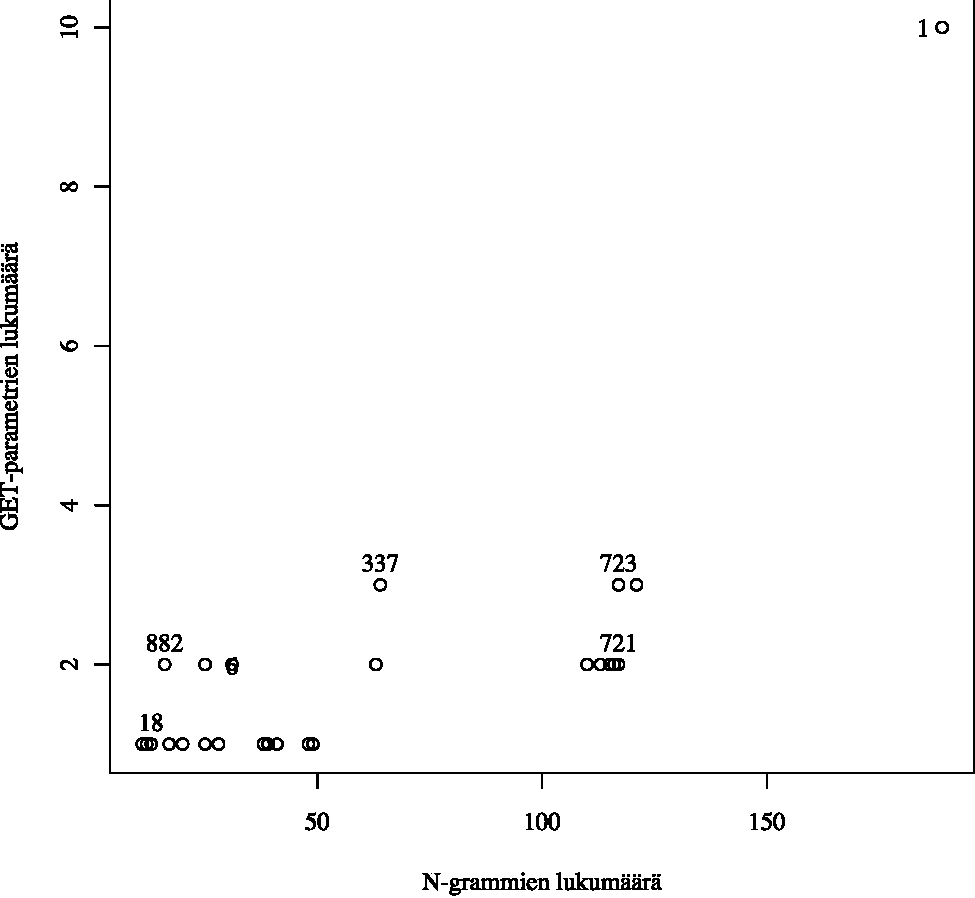
\includegraphics[width=13cm]{pics/service_resources.pdf}
\caption{Palvelun resurssien ominaisuudet.}
\label{service_resources}
\end{figure}

Analysoitavan palvelun eri resurssit on esitetty kuvassa
\ref{service_resources}. Kuvassa vaaka-\-akselina on käytetty
N-grammien lukumäärää ja pystyakselina GET-parametrien
lukumäärää. Resursseista valitsimme kuusi tarkempaan tarkasteluun ja
ne on merkitty kuvaajaan niiden resurssinumerolla.  Resurssit pyrimme
valitsemaan siten, että jokaisesta ryppäästä olisi yksi valittuna.

Palvelun jokaisesta resurssista muodostettiin aluksi diffuusiokuvaus
käyttäen edellä kuvatulla tavalla suodatettua aineistoa.
Analysoimalla saatua diffuusiokuvausta voitiin määrittää ne pisteet,
jotka oli luokiteltu poikkeaviksi siinä joukossa, jossa kyseisiä
pisteitä oli verrattu. 

Seuraavaksi lasketuista diffuusiokuvauksista muodostettiin
diffuusiokartta käytäen toista ja kolmatta ominaisvektoria. Koska
suuri määrä pisteitä sijoittui täsmälleen samoihin koordinaatteihin,
kartan luettavuuden parantamiseksi sirontakuvion pisteitä
``täristettiin''. Täristäminen suoritettiin lisäämällä
ominaisvektorien arvoihin normaalijakaumasta satunnaisesti poimittu
arvo. Normaalijakauman keskihajontana käytettiin yhtä prosenttia
akselin leveydestä. Kuvassa \ref{diffusio_1} nähdään edellä kuvatulla
tavalla muodostettu diffuusiokartta resurssista 1. Kuvaajasta voidaan
havaita, että muutamaa poikkeusta lukuunottamatta pisteet sijoittuivat
hyvin lähelle toisia.

Diffuusiokartta ei ole sellaisenaan kovinkaan havainnollinen, joten
jokaiselle pisteelle laskettiin vielä poikkeavuusluku. Se muodostettiin
summaamalla euklidinen etäisyys lähimpään kolmeen pisteeseen
diffuusiokuvauksen toisen, kolmannen ja neljännen ominaisvektorin
muodostamassa diffuusioavaruudessa. Tämän etäisyystiedon avulla voitiin piste
luokitella poikkeavuudeksi sekä piirtää poikkeavuuskartta.

% FIXME etäisyyskartta -> poikkeavuuskartta. Tuomon vinkki.

Kuvassa \ref{service_1} on resurssista 1 muodostettu poikkeavuuskartta. Kuvaajassa vaaka-akselille on sijoitettu resurssille kohdistuneet HTTP-kyselyt
ja pystyakselin mittana on poikkeavuus. Tässä pystyakseli ilmaisee sen kuinka poikkeava kukin piste on vertailujoukon sisällä. Jokaiselle kuvaajalle
on vielä määritetty keskihajonta ja raja-arvo, jonka ylittäneet pisteet merkitään poikkeaviksi. Tämä raja-arvo vaihtelee tapauskohtaisesti ja sen
arvo on kolme kertaa keskihajonta. Keskihajonta on merkitty kuvaajaan katkoviivalla ja raja-arvo yhtenäisellä viivalla. Esimerkiksi resurssin 1 
poikkeavuusskartassa \ref{service_1} on nähtävissä viisi poikkeavuudeksi merkittyä pistettä.

Jokainen diffuusiokartan luomiseen käytetytty piste pystytään
palauttamaan siihen HTTP-kyselyyn, josta se on
muodostettu. Esitetyissä kuvaajissa palauttamiseen tarvittavat tiedot
on merkitty niihin pisteisiin, jotka ylittävät raja-arvon. Otetaan
esimerkiksi kuvaajan \ref{service_18} ainoaksi merkitty poikkeama,
jolla on arvot ovat 7,3 ja 14594. Näistä ensimmäinen arvo ilmoittaa
sen tiedoston järjestysnumeron, josta kyseinen HTTP-kysely
löytyy. Seuraava luku puolestaan kertoo sen palvelimen
järjestysnumeron, johon kysely on ohjattu. Näiden kahden luvun avulla
voidaan yksilöidä tietty lokitiedosto. Viimeisin luku sisältää
rivinumeron kyseisen lokitiedoston sisällä.

\section{Tulokset}

Analysoitavassa materiaalissa resurssilla 1 \ref{service_1} oli viisi HTTP-kyselyä, jotka merkittiin poikkeaviksi. Tutkimalla diffuusiokuvauksen
luomiseen käytettyä lokia, ja palauttamalla HTTP-kyselyt alkuperäiseen muotoon, pystyimme paikallistamaan nämä kyselyt ja vertaamaan niitä lokin
muihin kyselyihin. Resurssin 1 tapauksessa kolme poikkeavaksi merkittyä kyselyä sisälsi sellaisen tunnistetiedon käyttäjistä, jota ei esiintynyt 
muissa kyselyissä. Kahdesta jäljelle jääneestä kyselystä yhdessä oli yritetty suoraan pyytää sellaista sivustoa, johon palvelu ei todennäköisesti
tarjonnut mahdollisuutta. Viimeisin kysely sitten... FIXME: Tarkistettava Joelilta onko tuossa joku bugi?

Kuvassa \ref{service_18} on nähtävillä resurssin 8 poikkeavuuskartta. Kyseisessä otannassa oli mukana 181 pistettä ja näistä yksi todettiin poikkeavaksi.
Resurssi 8 tarjosi vain staattista sisältöä, joten GET-parametrin jälkeistä kyselyosuutta ei HTTP-kyselyissä pitänyt olla. Poikkeavassa kyselyssä oli
GET-parametrin resurssipolun jälkeen kuitenkin kysymysmerkki, ja tämän perässä oli pyynnön tehneen alustan verkko-osoite. Poikkeavan kyselyn tunnistaminen
oli helppoa, sillä se oli ainoa kysely, jolle n-gram analyysi tuotti rivejä. Resurssille tehty kysely oli selkeästi virheellinen, sillä merkitty verkko-osoite 
oli privaattiverkon osoite. Kyselyssä käytetty alusta oli myös ainoa laatuaan.

Resurssisa 337 \ref{service_337} poikkeavuuksia havaittiin kuusi kappaletta. Näistä neljässä oli GET-parametrin jälkeen lisättynä samanlainen tunnistetieto
kuin resurssin 1 kolmessa havaitussa poikkeavuudessa. Yksi poikkeavuus taas oli saman käyttäjän aiheuttama kuin resurssilla 8, sillä kysely tuli samasta
verkko-osoitteesta ja näiden välillä ei ollut kuin muutama minuutti aikaa. Käytetty alusta oli myös ainoa laatuaan ja kyselyyn oli lisätty perään
sama verkko-osoite. Onkin hyvin todennäköistä, että pyydetyt palvelut eivät ole suunniteltu kyseiselle alustalle, jolloin kyselyiden oikeassa muodostuksessa ilmenee
virheitä. Viimeisessä poikkeavassa kyselyssä oli sitten muista eroava määrä avain-arvo pareja.

Kuvien \ref{service_721} ja \ref{service_723} poikkeavuudet aiheutuivat samaan tapaan ylimääräisestä tunnistetiedosta, joka oli lisätty kyselyiden perään. Kyselyt olivat selkeästi tulleet
saman välityspalvelun kautta, ja niistä jokainen oli tullut eri käyttäjältä. Tämä viittaisikin siihen, että kyseinen välityspalvelu olisi konfiguroitu virheellisesti. Tämän takia
sen kautta tulevat pyynnöt muodostettiin virheellisesti ja palvelimelle tulevia pyyntöjä ei pystytty käsittelemään oikein. Viimeisessä kuvassa \ref{service_882} resurssin poikkeama aiheutui siitä, 
että kyseinen HTTP-pyyntö oli ainoa, johon oli lisätty erillinen arvo. Muut käyttäjät ainoastaan latasivat saman tiedostoa ilman ylimääräisiä parametreja.. 

\begin{figure}[p]
\centering
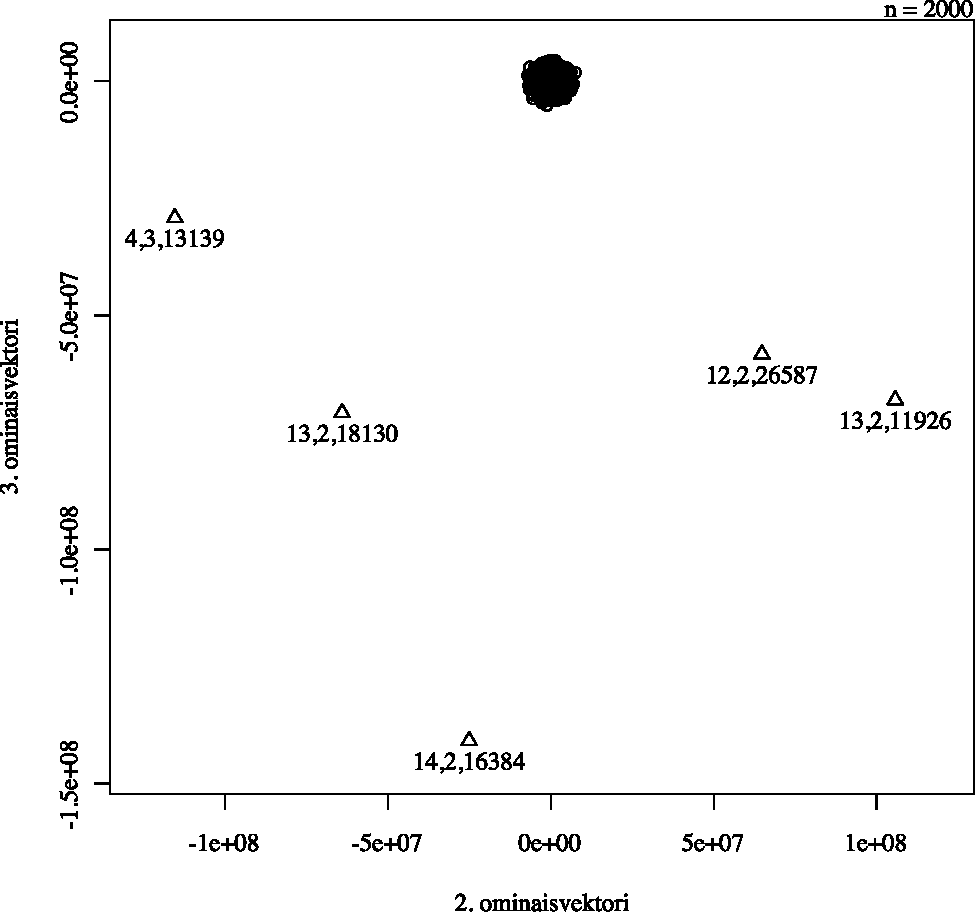
\includegraphics[width=11cm]{pics/diffuusiokuvat/service_1.pdf}
\caption{Resurssin 1 täristetty diffuusiokartta.}
\label{diffusio_1}
\end{figure}

\begin{figure}[p]
\centering
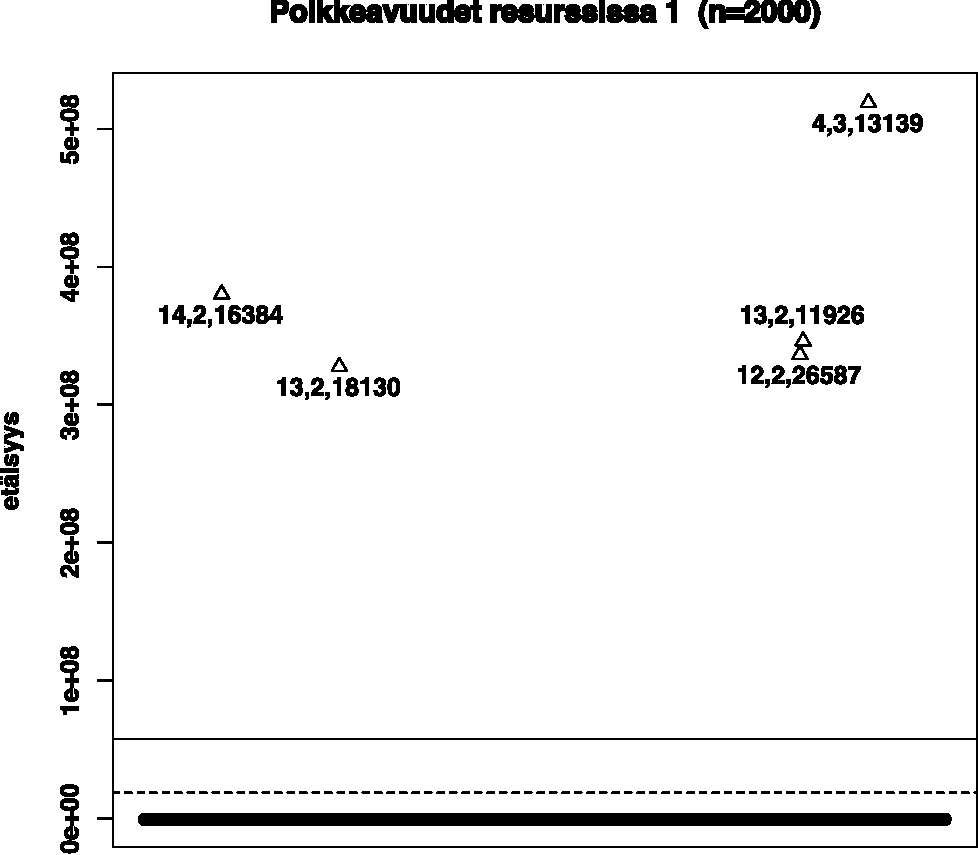
\includegraphics[width=11cm]{pics/tiheyskuvat/service_1.pdf}
\caption{Resurssin 1 poikkeavuuskartta.}
\label{service_1}
\end{figure}

\begin{figure}[p]
\centering
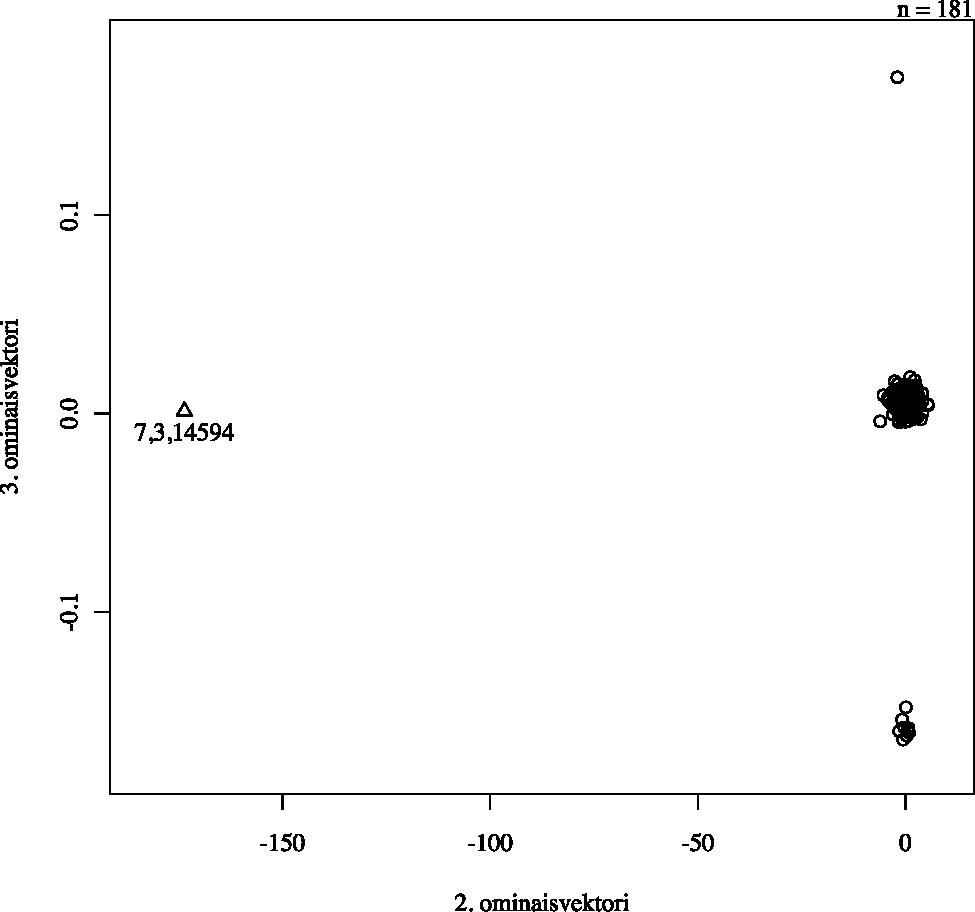
\includegraphics[width=11cm]{pics/diffuusiokuvat/service_18.pdf}
\caption{Resurssin 18 täristetty diffuusiokartta.}
\label{diffusio_18}
\end{figure}

\begin{figure}[p]
\centering
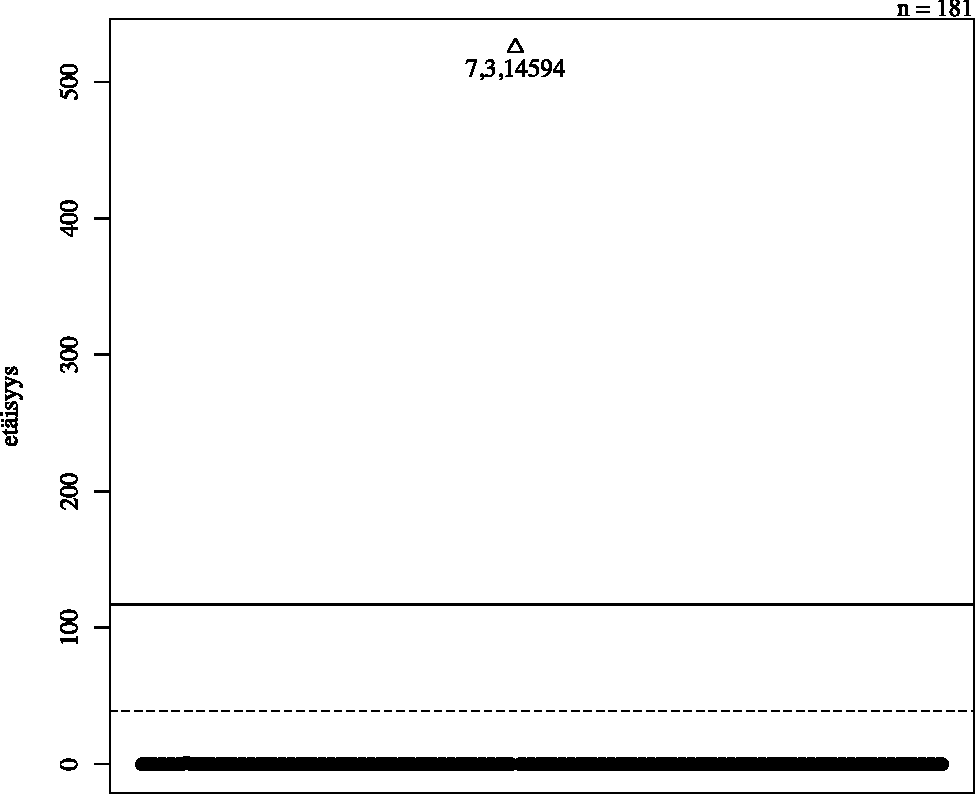
\includegraphics[width=11cm]{pics/tiheyskuvat/service_18.pdf}
\caption{Resurssin 18 poikkeavuuskartta.}
\label{service_18}
\end{figure}

\begin{figure}[p]
\centering
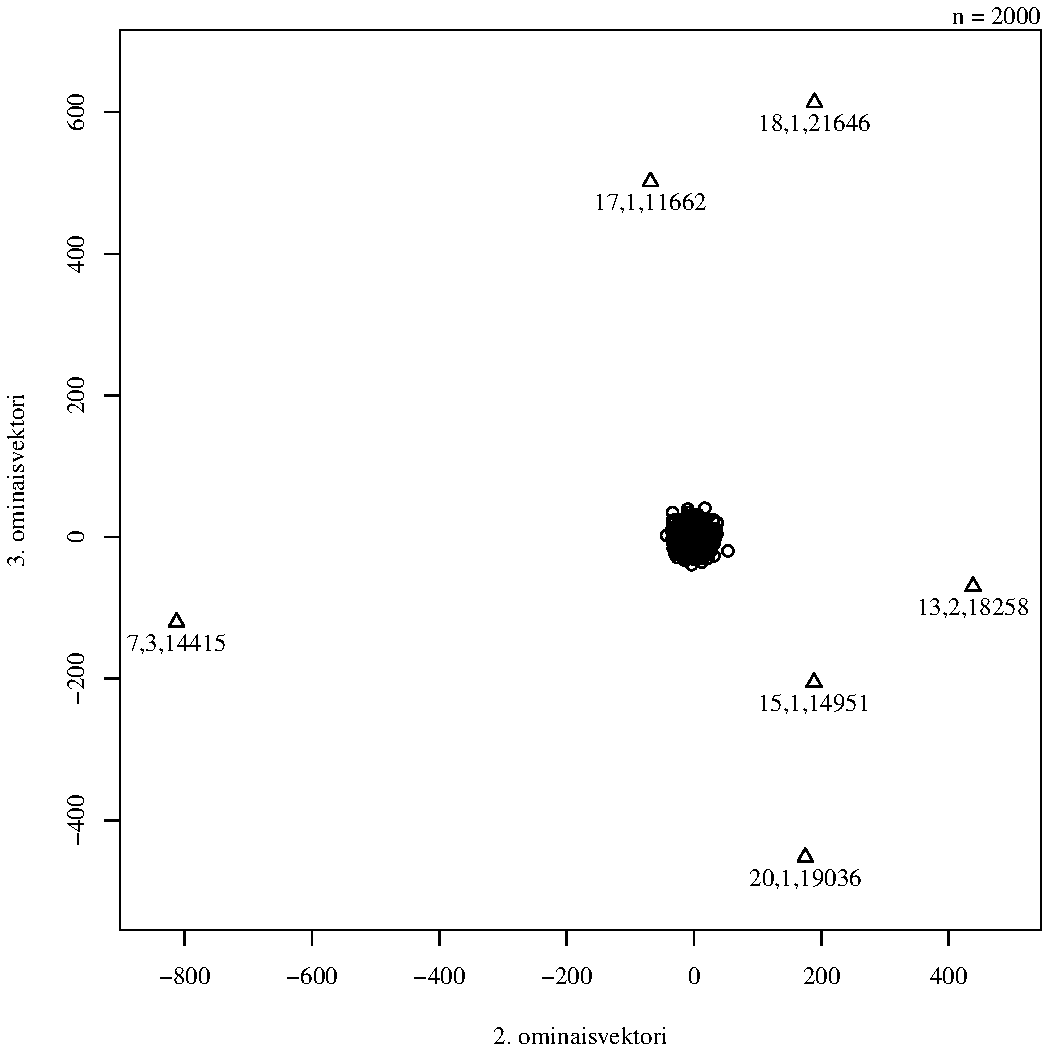
\includegraphics[width=11cm]{pics/diffuusiokuvat/service_337.pdf}
\caption{Resurssin 337 täristetty diffuusiokartta.}
\label{diffusio_337}
\end{figure}

\begin{figure}[p]
\centering
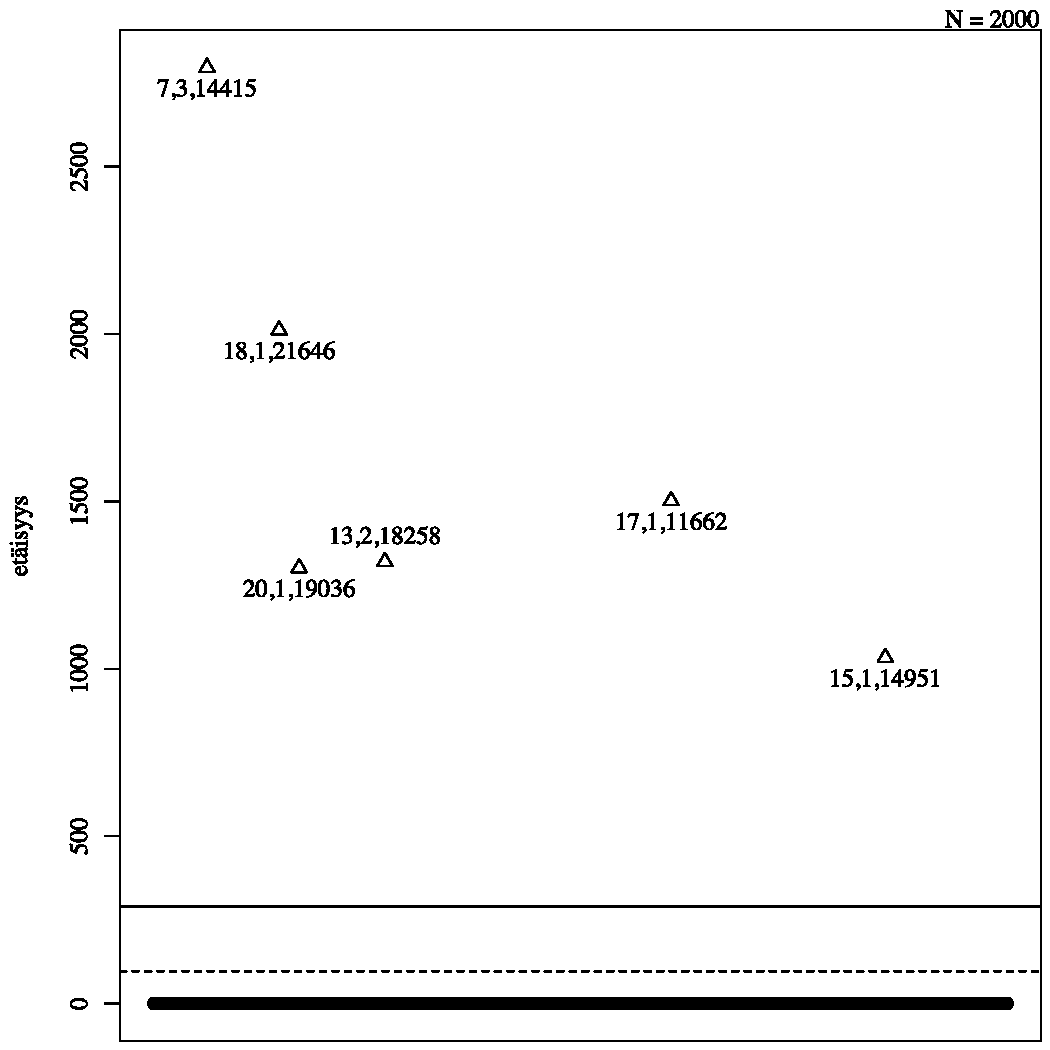
\includegraphics[width=11cm]{pics/tiheyskuvat/service_337.pdf}
\caption{Resurssin 337 poikkeavuuskartta.}
\label{service_337}
\end{figure}

\begin{figure}[p]
\centering
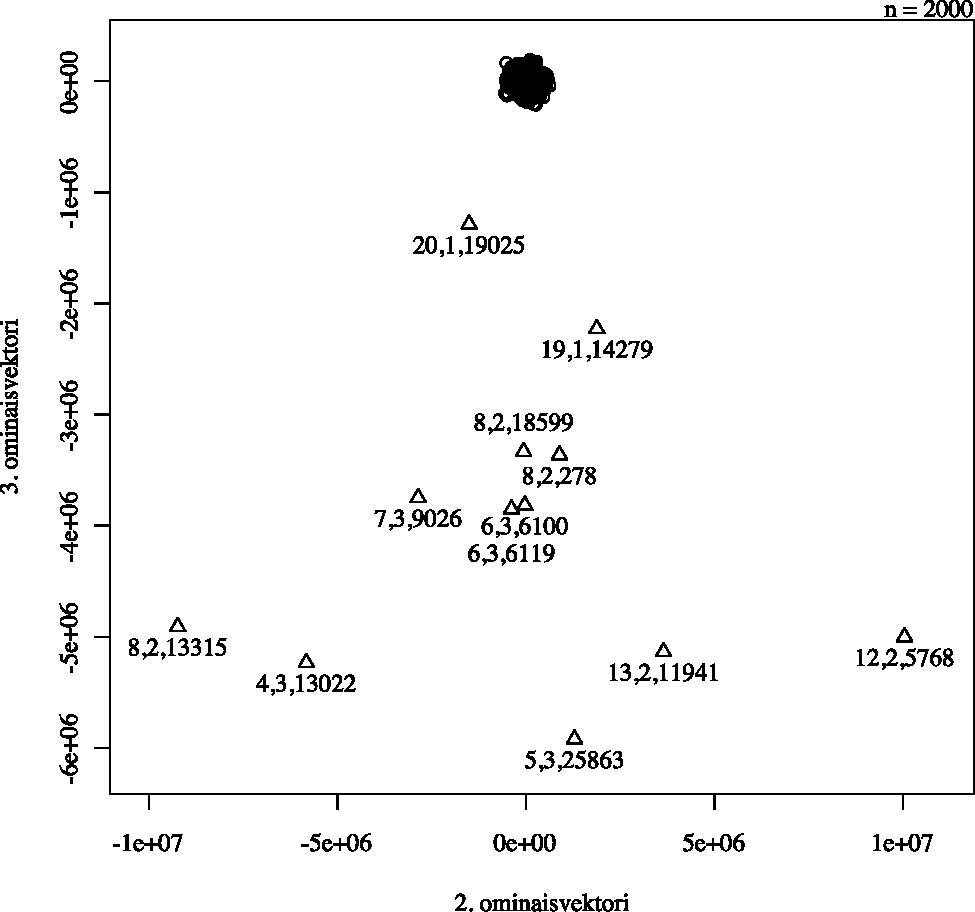
\includegraphics[width=11cm]{pics/diffuusiokuvat/service_721.pdf}
\caption{Resurssin 721 täristetty diffuusiokartta.}
\label{diffusio_721}
\end{figure}

\begin{figure}[p]
\centering
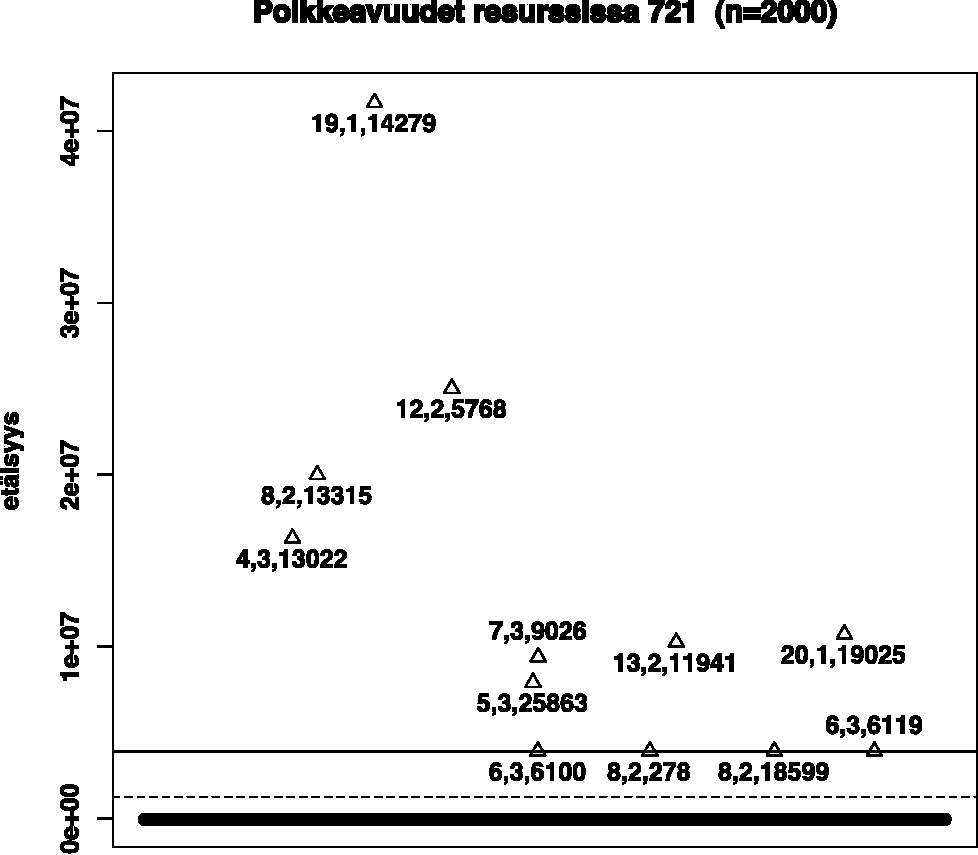
\includegraphics[width=11cm]{pics/tiheyskuvat/service_721.pdf}
\caption{Resurssin 721 poikkeavuuskartta.}
\label{service_721}
\end{figure}

\begin{figure}[p]
\centering
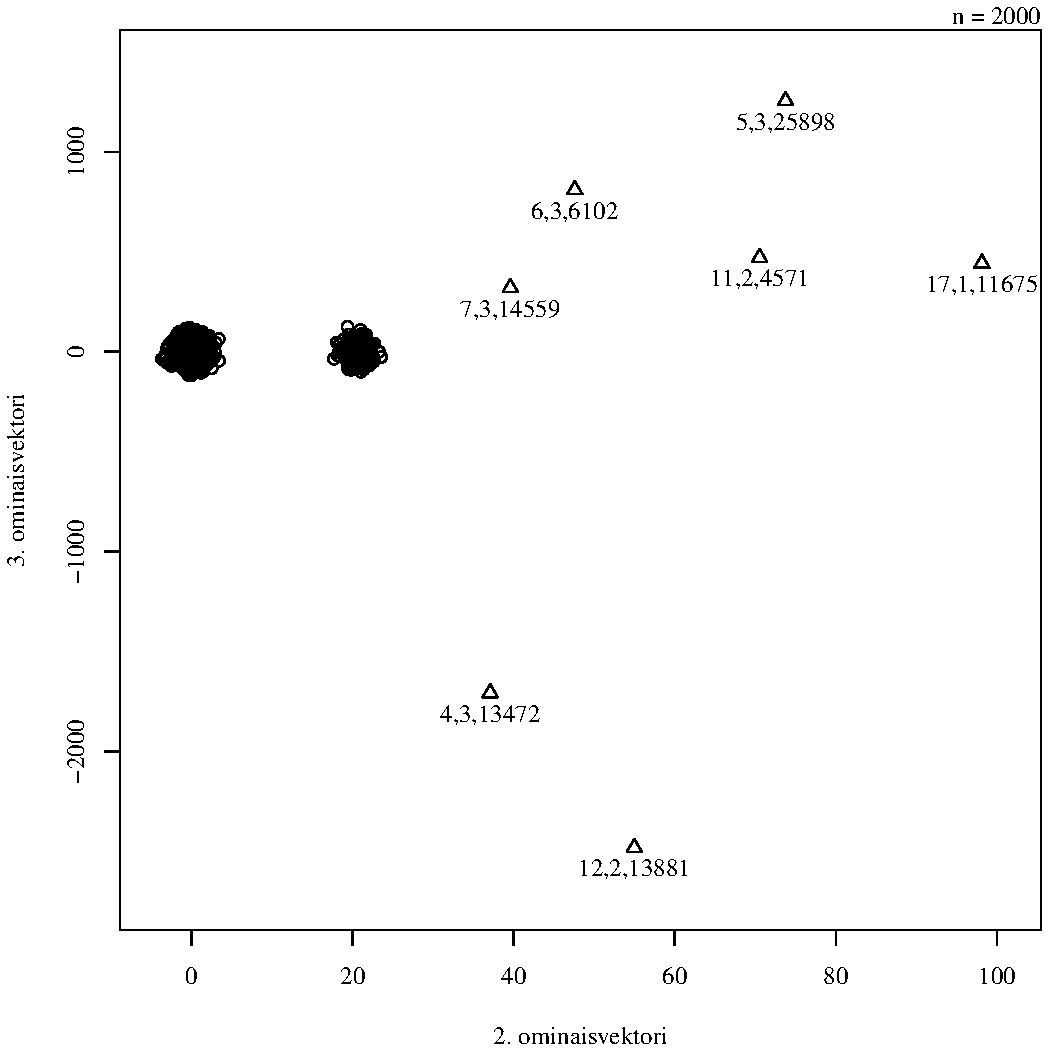
\includegraphics[width=11cm]{pics/diffuusiokuvat/service_723.pdf}
\caption{Resurssin 723 täristetty diffuusiokartta.}
\label{diffusio_723}
\end{figure}

\begin{figure}[p]
\centering
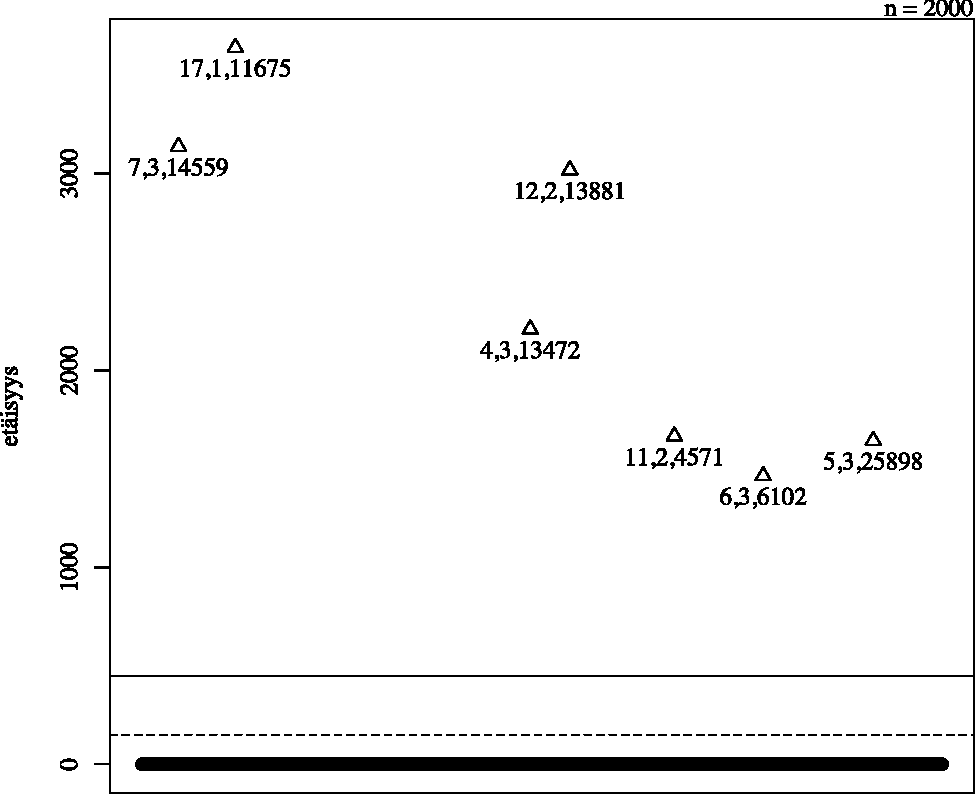
\includegraphics[width=11cm]{pics/tiheyskuvat/service_723.pdf}
\caption{Resurssin 723 poikkeavuuskartta.}
\label{service_723}
\end{figure}

\begin{figure}[p]
\centering
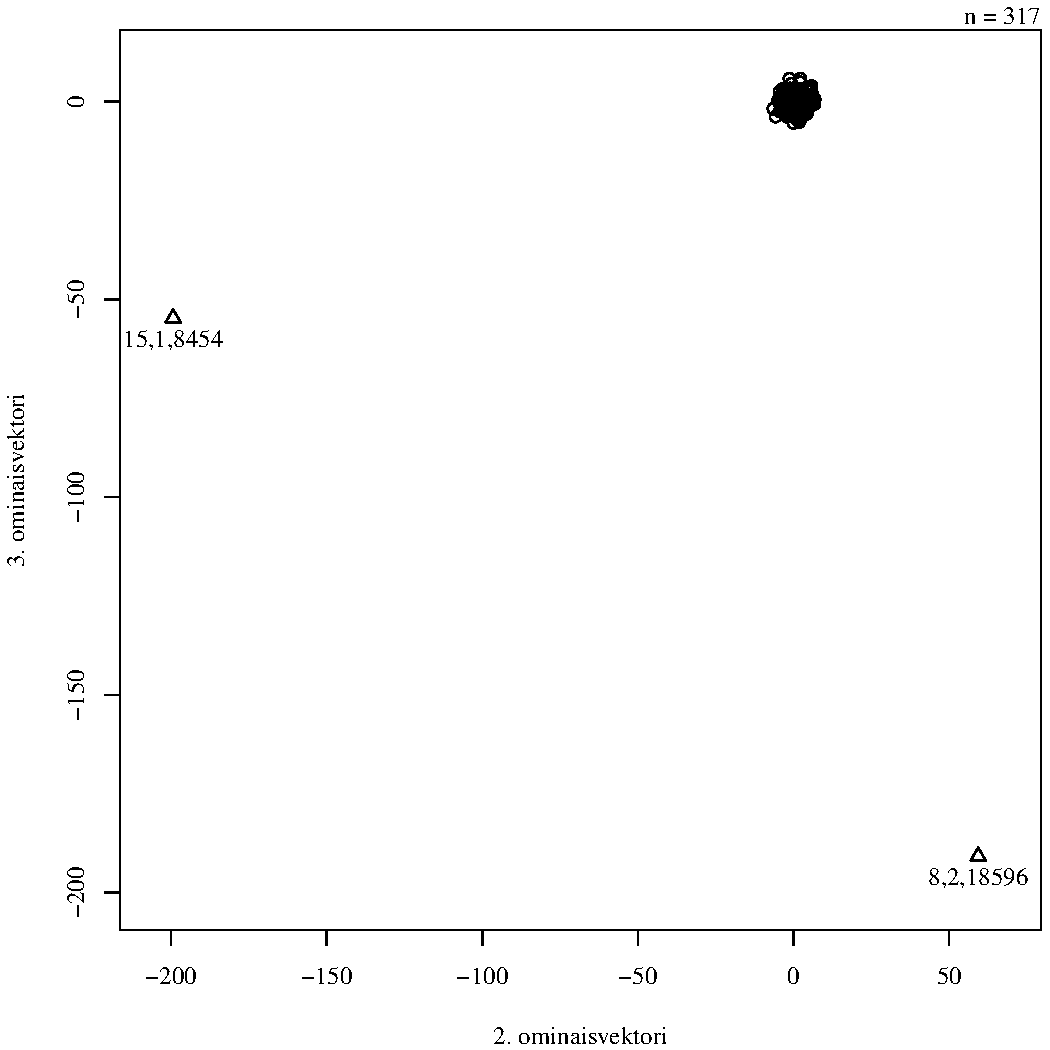
\includegraphics[width=11cm]{pics/diffuusiokuvat/service_882.pdf}
\caption{Resurssin 882 täristetty diffuusiokartta.}
\label{diffusio_882}
\end{figure}

\begin{figure}[p]
\centering
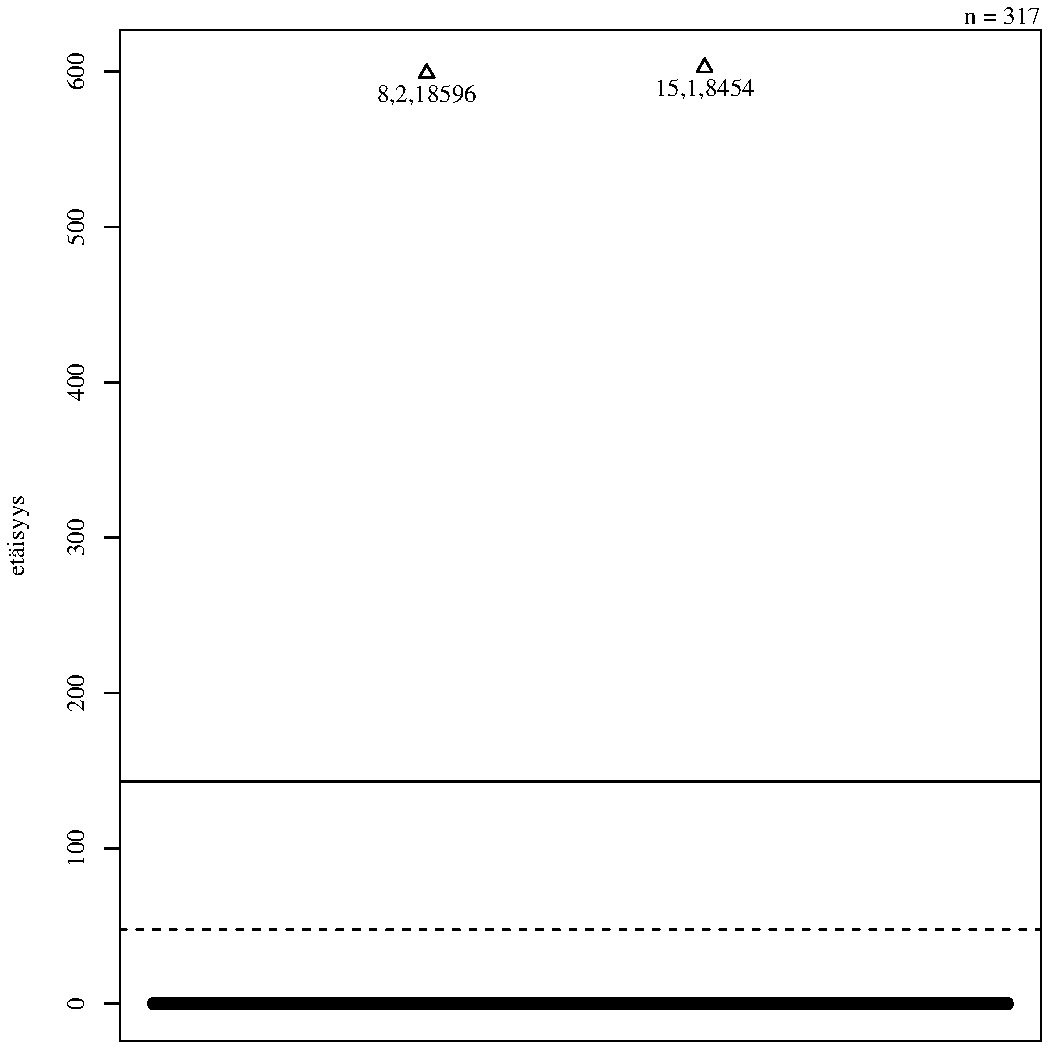
\includegraphics[width=11cm]{pics/tiheyskuvat/service_882.pdf}
\caption{Resurssin 882 poikkeavuuyskartta.}
\label{service_882}
\end{figure}

\section{Johtopäätöksiä ja kehitysideoita}

Analyysissä tuli hyvin esille se, että suurin osa liikenteestä oli hyvin samankaltaista. Tutkittavan materiaalin osalta tätä osattiin odottaa, mutta erilaisten pyyntöjen pieni määrä yllätti
siitä huolimatta. Ja vaikka kyseisestä otannasta ei varsinaisia tietoturvahyökäyksiä löydetty, olimme tyytyväisiä saatuihin tuloksiin. Tulokset osoittivat selkeästi sen, että esikäsittelijä toimi halutulla tavalla ja 
valittujen menetelmien avulla poikkeavat pyynnöt pystyttiin paikallistamaan. Myös todennäköisyys siihen, että analysoitavalle jaksolle olisi osunut jonkinlaisia tietoturvahyökkäyksiä, oli häviävän pieni
johtuen tiedon suuresta massasta. Kyseiset palvelut eivät muutenkaan olleet sellaisia, joihin hyökkääjillä olisi ollut suurta mielenkiintoa.  

Vaikka tässä työssä diffuusiokuvausten luomiseen käytettävien kyselyiden määrä rajoitti jonkin verran analyysin tekemistä, ei tämä käytännön ratkaisuissa muodostuisi ongelmaksi. Reaaliaikaisessa toteutuksessa
järjestelmälle opetetaan etukäteen normaali käyttäytyminen diffuusiokuvauksen avulla, jonka jälkeen uusien pisteiden paikka vertailujoukossa lasketaan yksitellen. Tällöin algoritmin käyttämä laskenta-aika
pysyy vakiona. Uudet pisteet voidaan projisoida diffuusiokuvaukseen esimerkiksi Nyströmin laajennuksen avulla, mutta tätä emme tähän työhön ottaneet enää mukaan. Menetelmä on kuitenkin hyvin tunnettu,
ja sitä on sovellettu monissa diffuusiokuvausten käyttöön pohjautuvissa tutkimuksissa.  

Seuraava looginen askel testauksissa olisi analysoida materiaalia rajatummalta alustalta ja lyhyemmältä ajanjaksolta. Esimerkiksi lokitiedot sellaisilta ajan hetkiltä, jolloin tietomurtoyritysten tiedetään tapahtuneen,
tarjoaisi erinomaiset puitteet testata tässä työssä käytettyjä ratkaisuja. Tätä kautta voitaisiin myös määrittää uusia parametreja, ja laajentaa käytettyjä menetelmiä. N-grammien lisäksi järjestelmä
voisi käyttää parametreina esimerkiksi samasta osoitteesta tulevien kyselyiden tiheyttä ja resurssipyynnöissä esiintyvien merkkien yleistä jakautumista. Käyttäjän IP-osoitteesta voitaisiin myös selvittää esimerkiksi
palveluntarjoaja, jonka kautta kysely tuli. Opetusjakson tarkempi määrittely tarjoaisi myös analyysin kannalta luotettavampaa tietoa. 

- Verkkokerroksen hyökkäykset jää huomaamatta. 

% -*- mode: LaTeX; coding: utf-8; -*-

\chapter{Yhteenveto}

TODO.


%\chapter{Introduction}


The structure of this thesis is following. In chapter
\ref{CHAPTER:EEG} the basics of EEG will be explained. Event-related
potentials (ERP) and their components are introduced in chapter
\ref{CHAPTER:ERP} along with a special case of ERP, mismatch
negativity (MMN). After the basic biomedical concepts the focus will
shift to data analysis methods. Chapter \ref{CHAPTER:LINEAR} takes a
brief look at the more traditional linear time-frequency methods used
in EEG analysis. Empirical mode decomposition and intrinsic mode
functions are discussed in chapter \ref{CHAPTER:EMD}. Theoretical
background behind Hilbert transform and Hilbert spectrum are
introduced in chapter \ref{CHAPTER:HT_HS}.
Jeejee.

%\chapter{Electroencephalography}
\label{CHAPTER:EEG}

During the 1990s EEG was used increasingly with alternative neuroimagining techniques. Intensive care units were deployed to monitor EEG in real time in hospital environments. Complementary methods were invented but EEG has superior time resolution and remains in use \cite{LUCK2005, SWARTZ1998b}. 

\section{Brain rhythms}

Some recurrent parts of EEG have a clear origin and frequency. These repeating rhythms can be rather easily observed and they are associated with different states of alertness. For these reasons the rhythms were discovered early in EEG research and have been used as diagnostic tools and ways to characterize an EEG waveform. The most common rhythms are historically named beta ($13-30Hz$), alpha ($8-13Hz$), theta ($4-8Hz$) and delta ($0.5-4Hz$) \cite[pp. 10--12]{SANEI2007}. 

%% \begin{figure}[htp]
%% \centering
%% \includegraphics[width=150pt]{pics/electrode_positions.pdf}
%% \caption[Conventional electrode positioning]{Conventional 10--20 electrode positions. Figure adapted from Sanei and Chambers \cite[p. 16]{SANEI2007}.}
%% \label{ELECTRODE_POSITIONS}
%% \end{figure}

From the probability point of view a stochastic process $X=X(t)$ is stationary if vector $\mathbf{X}(t)=(X(t_1), X(t_2), \dots, X(t_n))$ has the same cumulative distribution as $\mathbf{X}(t+s)=(X(t_1+s),X(t_2+s),\dots,X(t_n+s))$, that is, 

\begin{equation}
F_{\mathbf{X}(t+s)}(\textbf{x}) = F_{\mathbf{X}(t)}(\textbf{x})
\label{CUM_DIST}
\end{equation}

The algorithm consists of the following steps: 

\begin{enumerate_no_space}
\item find the extrema of $x(t)$ \label{FIRST}
\item create envelope $E_u(t)$ by interpolating between the maxima ($E_l(t)$ for minima)\label{ENV}
\item mean envelope $m(t) = (E_u(t)+E_l(t))/2$
\item extract the details $c(t) = x(t) - m(t)$ \label{DETAIL}
\item go to \ref{ENV} until $c(t)$ is considered IMF \label{SIFT}
\item iterate from the start with the residue signal $r(t) = x(t) - c(t)$.
\end{enumerate_no_space}

Jee.

\begin{table}
\centering
\begin{tabular}{c c c c c c c}

\textbf{Group} & \textbf{Number} & \textbf{Boys} & \textbf{Girls} & \textbf{Min age} & \textbf{Mean age} & \textbf{Max age} \\ \hline
RD      & 16 & 11 & 5  & 8y8m & 12y2m  & 14y2m \\
ADHD    & 16 & 15 & 1  & 9y2m & 11y0m  & 13y5m \\
Control & 66 & 41 & 25 & 8y2m & 11y11m & 16y9m \\

\end{tabular}
\caption{Subjects were divided into three groups}
\label{SUBJECTS}
\end{table}


\begin{thebibliography}{99}

\bibitem{IDS}
S. Mukkamala, A.H. Sung, \textit{A Comparative Study of Techniques for Intrusion Detection} kirjassa Tools with Artificial Intelligence, 
15th IEEE International Conference, 2003.

\bibitem{WEBS}
B. Shweta, \textit{Web Security Basics}, Course Technology, 2002.

\bibitem{DDOS}
D. Dittrich, S. Dietrich, J. Mirkovic, P. Reiher, \textit{Internet Denial of Service: Attack and Defence Mechanisms}, Prentice Hall PTR, 2004.

\bibitem{DDOSb}
S. Ranjan, R. Swaminathan, M. Uysal, E. Knightly, \textit{DDoS-Resilient Scheduling to Counter Application Layer Attacks under Imperfect Detection},
Infocom 2006, 25th IEEE International Conference on Computer Communications, 2006.

\bibitem{FBI}
FBI, \textit{Wanted by the FBI - Saad Echouafni}, <URL: \texttt{http://www.fbi.gov/wanted/fugitives/cyber/echouafni\_s.htm}>, viitattu 27.10.2009.

\bibitem{CERT}
CERT, \textit{Denial of Servce}, saatavilla WWW-muodossa <URL: \texttt{http://www.cert.org/tech\_tips/denial\_of\_service.html}>, viitattu 20.10.2009.

\bibitem{STACK}
R. Bandes, B. Franklin, M. Gregg, G. Mays, C. Ries, S. Watkins, \textit{Hack the Stack}, Syngress Publishing Inc, 2006. 

\bibitem{IDSb}
R. Lippmann, D. Stetson, S. Webster, \textit{The Effect of Identifying Vulnerabilities and Patching Software on the Utility of Network Intrusion Detection},
kirjassa Recent Advances in Intrusion Detection, 2002.

\bibitem{TCP}
K. Kaario, \textit{TCP/IP-verkot}, Docendon, 2001.

\bibitem{CVE}
CVE, <URL: \texttt{http://www.cve.mitre.org/cve}>, viitattu 29.10.2009.

\bibitem{SYM}
Symantec, \textit{Symantec Internet Security Threat report. Trends for July-December 2007}, saatavilla WWW-muodossa
<URL: \texttt{http://www.symantec.com/business/index.jsp}>, viitattu 1.12.2009.

\bibitem{SYM2}
Symantec, \textit{Symantec Global Internet Security Threat Report. Trends for 2008}, saatavilla WWW-muodossa <URL: \texttt{http://www.symantec.com/business/index.jsp}>,
viitattu 1.12.2009.


\bibitem{U2R}
Z. Bankovic, S. Bojanic, O. Nieto-Taladriz, A. Badii, \textit{Increasing Detection Rate of User-to-Root Attacks Using Genetic Algorithms}, 
Emerging Security Information, Systems, and Technologies, 2007.

\bibitem{SQL SS}
C. Andrews, D. Litchfield, \textit{SQL Server Security}, McGraw-Hill Osborne, 2003.

\bibitem{WEB2}
R. Cannings, H. Dwidedi, Z. Lackey, \textit{Hacking Exposed Web 2.0: Web 2.0 Security Secrets and Solutions}, McGraw-Hill Companies, 2008.

\bibitem{WEB2b}
S. Shreeraj, \textit{Web 2.0 Security: Defending Ajax, RIA and SOA}, Course Technology, 2007.

\bibitem{WEB2c}
G. Lawton, \textit{Web 2.0 Creates Security Challenges}, Computer-IEEE Computer Society, saatavilla WWW-muodossa <URL: \texttt{http://www.computer.org}>,
viitattu 5.11.2009.

\bibitem{SOA}
IBM Redbooks, \textit{Patters: Service-Oriented Architecture and Web Services}, IBM, 2004.

\bibitem{Hacking}
S. McClure, J. Scambray, G. Kurtz, \textit{Hacking Exposed (5th Edition)}, McGraw-Hill Osborne, 2005.

\bibitem{XSS}
XXSed, <URL:\texttt{http://http://www.xssed.com/archive/special=1}>, viitattu 2.12.2009.

\end{thebibliography}


\appendix

%\chapter{Published article}
%
%\includepdf[pages=-]{published_article.pdf}

\end{document}
